%\documentclass{cumcmthesis}
\documentclass[withoutpreface,bwprint]{cumcmthesis} %去掉封面与编号页,电子版提交的时候使用。


\usepackage[framemethod=TikZ]{mdframed}
\usepackage{url}   % 网页链接
\usepackage{subcaption} % 子标题
\title{华中杯数学建模}
\tihao{A}



\begin{document}
	
 \maketitle

%摘要

 \begin{abstract}

本文通过对实际太阳运动轨迹的建模,计算在不同角度下光伏板法向量与各个时间段太阳光方向向量之间的角度关系,综合考虑了太阳辐射能量、光伏转化效率、光伏储存效率,添加了相关文献中的各项参数,总结出光伏板角度与接收到太阳辐射总能量的模型,对于安装光伏板的朝向角度有一定的指导价值。

针对问题一,由于题目所给数据间隔较大,同时也是为了给后续运算做准备,我们对数据进行插值,从而提高精度。由于太阳光强的变化宏观上是一个连续过程,所以为了避免龙格现象,提升插值精度,使插值结果更平滑,我们采用三阶样条插值,使得插值结果在节点附近相对平滑。当插值获得数据后,我们建立三维坐标系,通过 Klein-Theilacker 模型与物理学投影,研究不同$\theta$下,最终的最大太阳直射强度和太阳直射辐射总能量。

针对问题二,我们在问题一的基础上,由于已经通过三维样条插值,获得了较高精度的数据,所以我们直接遍历所有的$\theta$和$\mu$从而得到最佳角度。

针对问题三,我们在之前模型的基础上,查询文献,引入更多物理参数——电池的储存效率、光伏板光伏转化效率来修正模型。为了综合考虑路灯蓄电池的储电效率高和储电量大这两个目标,来确定光伏板固定安装的最优朝向,我们采用了TOPSIS评价的方法来考虑不同朝向下的优劣;同时,为了减少评价的主观性,我们引入了熵权法来得到TOPSIS的权重。最后,当我们获得了最佳安装角度后,利用模型即可计算得到晴天条件下光伏板受到的太阳直射辐射日均总能量和太阳直射辐射。

本文综合Klein-Theilacker模型,熵权法+TOPSIS方法等模型,借助Excel,Pyhon 等软件运算、作图,对光伏板摆放角度与辐射能量的分析与评价问题进行了多角度的建模分析,并给出了综合角度与光伏板物理特性获得的最佳模型。文章最后对模型的适用范围作出了推广,在实际应用中有一定的参考价值。


\keywords{样条插值 \quad Klein-Theilacker模型\quad 熵权法 \quad TOPSIS方法}
\end{abstract}



%目录
\tableofcontents

\newpage


\section{问题重述}

太阳能路灯由太阳能电池板(也称光伏板)组件部分、LED灯头、控制箱、市电辅助器和灯杆等几部分构成。由于光伏板利用光伏效应接收太阳辐射能并转化为电能输出,并且经过充放电控制器储存在蓄电池中,所以,对光伏转化效率影响最大的的是光伏板和蓄电池。而光伏板获得太阳辐射能量的多少受到安装光伏板的朝向的直接影响;同样地,蓄电池转化、储存电能的效率受到太阳直射强度,也会受到安装光伏板的朝向的影响。所以,为了能使路灯在一天内获得最多的太阳能,我们研究太阳能路灯光伏板的朝向设计问题。

题目已经给出某城区晴天状况下测得地表水平面受到的太阳直射强度值,通过这些数据,我们将解决以下问题:

\begin{enumerate}
	\item 计算2025年每月15日,在晴天条件下,该城区一块面积为$1m^{2}$的光伏板朝向正南方且水平倾角分别为$20^{\circ}$、$40^{\circ}$、$60^{\circ}$时受到的最大太阳直射强度和太阳直射辐射总能量
	
	
	\item 当光伏板受到的太阳直射辐射总能量最大时,路灯蓄电池有储电量最大时,设计该城区固定安装太阳能光伏板的朝向,使光伏板在晴天条件下受到的太阳直射辐射日均总能量最大
	
	
	\item 当路灯蓄电池有储电量不在太阳直射辐射总能量最大时最大,而是光板受到太阳直射强度过低时,它转换电能的效率也很低;而当光伏板受到太阳直射强度过高时,它转换电能实现储电的效率也会受到限制。综合考虑路灯蓄电池的储电效率高和储电量大这两个目标,设计光伏板固定安装的最优朝向,并计算晴天条件下光伏板受到的太阳直射辐射日均总能量和太阳直射辐射
	
\end{enumerate}



\section{问题分析}



\subsection{问题一:数据插值与问题求解}

如图\ref{fig:001}所示,由于太阳半径远大于地球半径,并且光伏板的面积远小于地球面积,所研究的太阳光可以看作地球上一点所接收的光,为平行光。并且,由于地球绕太阳的轨道近似于圆轨道,具有对称性,所以认为轨道各处所接收到的太阳辐射强度相同,光伏板能接收到的辐射能量只与太阳高度角、以及光伏板摆放的角度有关。

对于这样一个对光伏板平面,我们建立坐标系,对太阳辐射能与角度关系进行研究。由于所给数据间隔过大,所以先进行插值提高精度,然后由物理学公式和Klein-Theilacker模型进行建模。
\begin{figure}
	\centering
	\begin{minipage}[c]{0.48\textwidth}
		\centering
		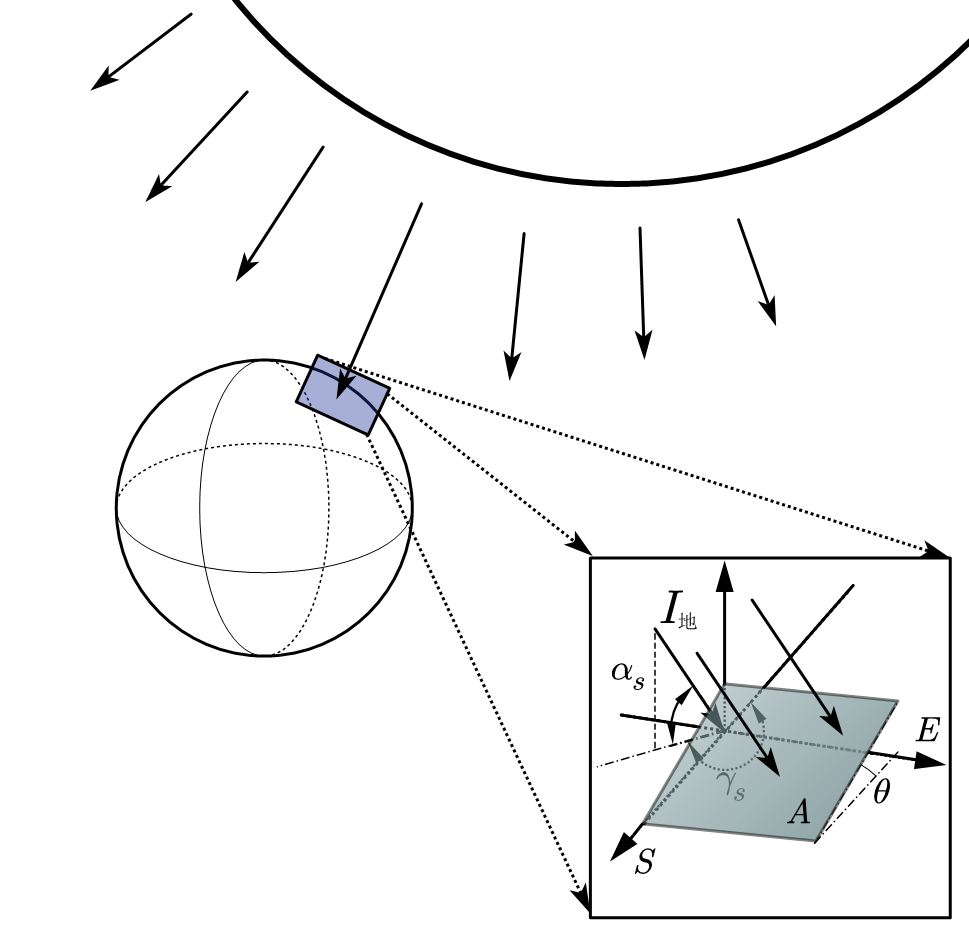
\includegraphics[height=0.2\textheight]{img2.png}
		\subcaption{太阳辐射地球示意图}
		\label{fig:001}
	\end{minipage}
	\begin{minipage}[c]{0.48\textwidth}
		\centering
		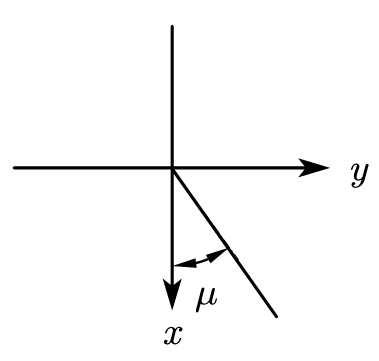
\includegraphics[height=0.2\textheight]{list1.png}
		\subcaption{光伏板坐标系}
	\end{minipage}
	\caption{问题一分析}
\end{figure}


\subsection{问题二:朝向设计与误差修正}

在问题一分析的基础上,已知对光伏转化效率影响最大的的是光伏板和蓄电池,如果假定果光伏板受到的太阳直射辐射总能量最大时,可使路灯蓄电池储电量最大,那么显然,当太阳直射辐射总能量最大时,所收集的能量也就最大。所以问题二中,在问题一的模型的基础上,只需要讨论$\theta_{k}$和光照强度变化而导致的太阳直射辐射总能量的变化。但是,由于每天的日照时长存在不同,所以额外考虑这一方面的误差,查找文献后,用一年中日均的光照时长来修正答案。

\subsection{问题三:转化率与储存率添加}

在问题二分析的基础上,考虑光伏板受到的太阳直射强度影响光伏转化效率、电池存储效率,所以辐射总能量最大时,路灯蓄电池储电量不一定最大。此时,我们要考虑综合路灯蓄电池的储电效率高和储电量大这两个目标。由于当光板受到太阳直射强度过低时,它转换电能的效率也很低;而当光伏板受到太阳直射强度过高时,它转换电能实现储电的效率也会受到限制。理想的情况是,光伏板受到太阳直射强度上午大于$150W/m^{2}$、下午大于$100W/m^{2}$的时间尽可能长,在此基础上,我们搜集文献,量化光照强度与效率的之间的数学关系。然后为了求得最有解,故采用TOPSIS评价综合考虑光照强度、转化效率、储存效率三个方面,并且采用熵权法客观求得三者的权值,找到能使日均辐射总能量最大的最优的$\theta$。



\newpage



\section{符号说明}

\begin{table}[!htbp]
    \caption{符号与常数}\label{tab:001} \centering
    \setlength{\tabcolsep}{15pt}
    \begin{tabular}{ccc}
        \toprule[1.5pt]
        符号 & 含义 & 单位或常数值\\
        \midrule[1pt]
        D & 以春分为起始的的第D天数 & 天\\
        ST & 当前时间 & h\\
        $I_{\mbox{外}i}$ & 第i周大气层外层平均太阳能辐射强度 & $kW/m^{2}$\\
        $\theta_{k}$ & 光伏板水平俯仰角 & $^{\circ}$\\
        $h$ & 大气层厚度 & $1000km$\\
        $I_{STC}$ & 标准太阳能辐射强度 & $1000W/m^{2}$\\
        $\eta_{STC}$ & 标准测试下的发电效率 & $15\%(T=25^{\circ}C)$\\
        $\alpha$ & 光伏转化效率系数 & $0.001$\\
        $\beta$ & 光电转化效率与光强系数 & -\\
        $\eta_{t}$ & 发电效率 & -\\
        $\eta_{at}$ & 大气透射率 & -\\
        $\eta_{\cos}$ & 余弦效率 & -\\
        $\Delta I$ & 辐射衰减变化量 & -\\
        $k$ & 区域衰减系数 & -\\
        $P_{\mbox{放}}$ & 单位面积放电功率 & $W$\\
        $P_{\mbox{储}}$ & 单位面积储电功率 & $W$\\
        $I_{\mbox{地5月15}}$ & 每阶段5月15日太阳直射辐射 & $W/m^2$\\
        $E_{\mbox{光}}$ & 太阳直射辐射总能量 & $J$\\
        $C$ & 储电量 & $J$\\
        $A$ & 光伏板面积 & $1m^{2}$\\
        $\overline{H_{T}}$ & 倾斜面上的太阳总辐射量 & $J$\\
        $\overline{R}$ & 倾斜面月平均辐照量与水平面月平均辐照量之比 & $J$\\
        $\overline{H}$ & 水平面上的太阳总辐照量 & $J$\\
        \bottomrule[1.5pt]
    \end{tabular}
\end{table}

\bigskip













\section{模型假设}

\begin{assumption}
	只考虑太阳能直射辐射
	\label{asu:001}
\end{assumption}
太阳能辐射由直射辐射和散射辐射组成和散射辐射组成,其中直射辐射对聚集太阳能系统起到了至关重要的影响。
\begin{assumption}
	太阳光近似为平行光
	\label{asu:002}
\end{assumption}
由于太阳半径远大于地球,所以辐射到地球的光线可以近似为平行光。
\begin{assumption}
	地球绕太阳公转的轨道几乎是一个圆形,太阳光的入射角度变化非常微小,日均的数据具有普遍性
	\label{asu:003}
\end{assumption}
在地球表面的大部分地区,太阳光到达时可以被视为近似平行的,并且由于太阳光线看作均匀的,所以各个方向发出的光线都相同,轨道各处接收到的光线无区别。
\begin{assumption}
	该地的云层组成含量一直保持不变,云层对阳光直射辐射的削减能力只与云层高度和阳光直射辐射有关
	\label{asu:004}
\end{assumption}
由于本问题只研究晴天条件下的模型,所以模型可以忽略云层等的影响


\section{模型的建立与求解}
\subsection{问题一}

由于所给数据间隔过大,所以先进行插值提高精度。由于这是一个物理过程,所以对数值平稳性要求较高,所以我们采取三维样条插值,以下为插值结果:

\begin{figure}[!h]
	\centering
	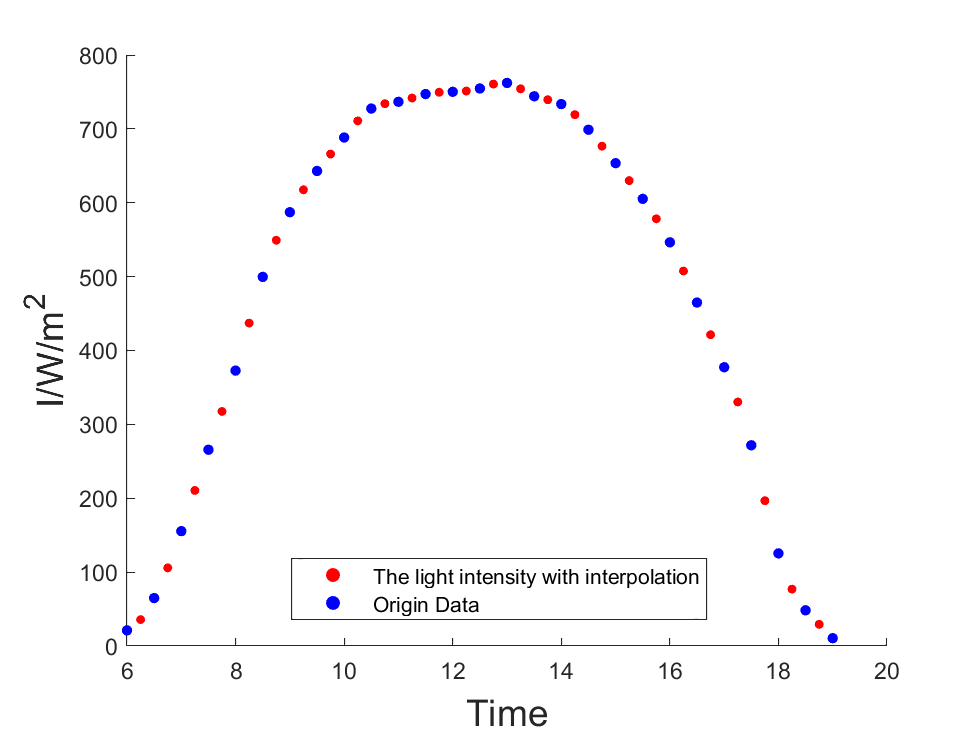
\includegraphics[width=.6\textwidth]{插值.png}
	\caption{插值结果}
	\label{fig:002}
\end{figure}

由Klein-Theilacker模型\cite{7},结合物理学公式,由假设\ref{asu:001}不考虑漫反射,假设\ref{asu:004}忽略气象因素只考虑晴天条件,故直接投影可求得比例系数$\overline{R}$。

\begin{equation}
	\overline{H_{T}} = \overline{R} \times \overline{H}
	\label{eq:001}
\end{equation}

太阳在一年中的运动轨迹是由地球的自转和公转引起的,其在地面上的位置随着时间不断变化,其变化轨迹被称为太阳的视运动轨迹。为了表述的方便,我们可以使用地坪坐标系来得到太阳的高度角$\alpha$和方位角$y$,进而确定太阳的方位。太阳时角是指日面中心的时角,即从观测点天球子午圈沿天赤道量至太阳所在时圈的角距离。当地时间12时为$\theta$,往后1小时+15度,往前1小时-15度可以由公式得出:
\begin{equation}
	\omega = \frac{\pi}{12}(ST - 12)
	\label{eq:002}
\end{equation}

其中,ST为当地时间。

太阳赤纬角是指太阳光线与地球赤道面之间的夹角,取值范围在-23.5°到23.5°之间,分别对应着夏至和冬至时太阳在天空中的最高点。它可以由如下公式得出:
\begin{equation}
	\sin\delta = \sin \frac{{2}\pi D}{365}\sin\left(\frac{2\pi}{360} \times 23.45\right)
	\label{eq:003}
\end{equation}

其中,D为以春分作为第0天起算的天数。

太阳高度角指太阳光的入射方向和地平面之间的夹角,简称太阳高度,如图所示,公式如下:
\begin{equation}
	\sin\alpha_{S} = \cos \delta \cos \phi \cos \omega + \sin \delta \sin \phi
	\label{eq:004}
\end{equation}

其中,$\phi$在当地纬度。

太阳方位角为从目标位置的北方沿着地平线顺时针到太阳光线在地面投影之间的角,如下:
\begin{equation}
	\cos y_{s} = \frac{ \sin \delta - \sin \alpha_{s} \sin \phi}{\cos \alpha_{s}\cos \phi}
	\label{eq:004}
\end{equation}

太阳能路灯光伏板吸收太阳能进行发热发光的关键在于光伏板对太阳直射辐射强度的吸收。为了更好描述这个工作流程,我们建立了路灯所处地面的坐标系XYZ,令路灯的中心位置为原点О,以正南方向为X轴的正方向,以正东方向为Y轴的正方向,以垂直地面向上方向为Z轴的正方向,建立路灯坐标系XYZ。这样太阳直射辐射就可以用向量来表示,而光伏板的朝向也可以用光伏板的面法向量来表达。太阳直射的方向向量和光伏板的面法向量如下图:

\begin{figure}[!h]
	\centering
	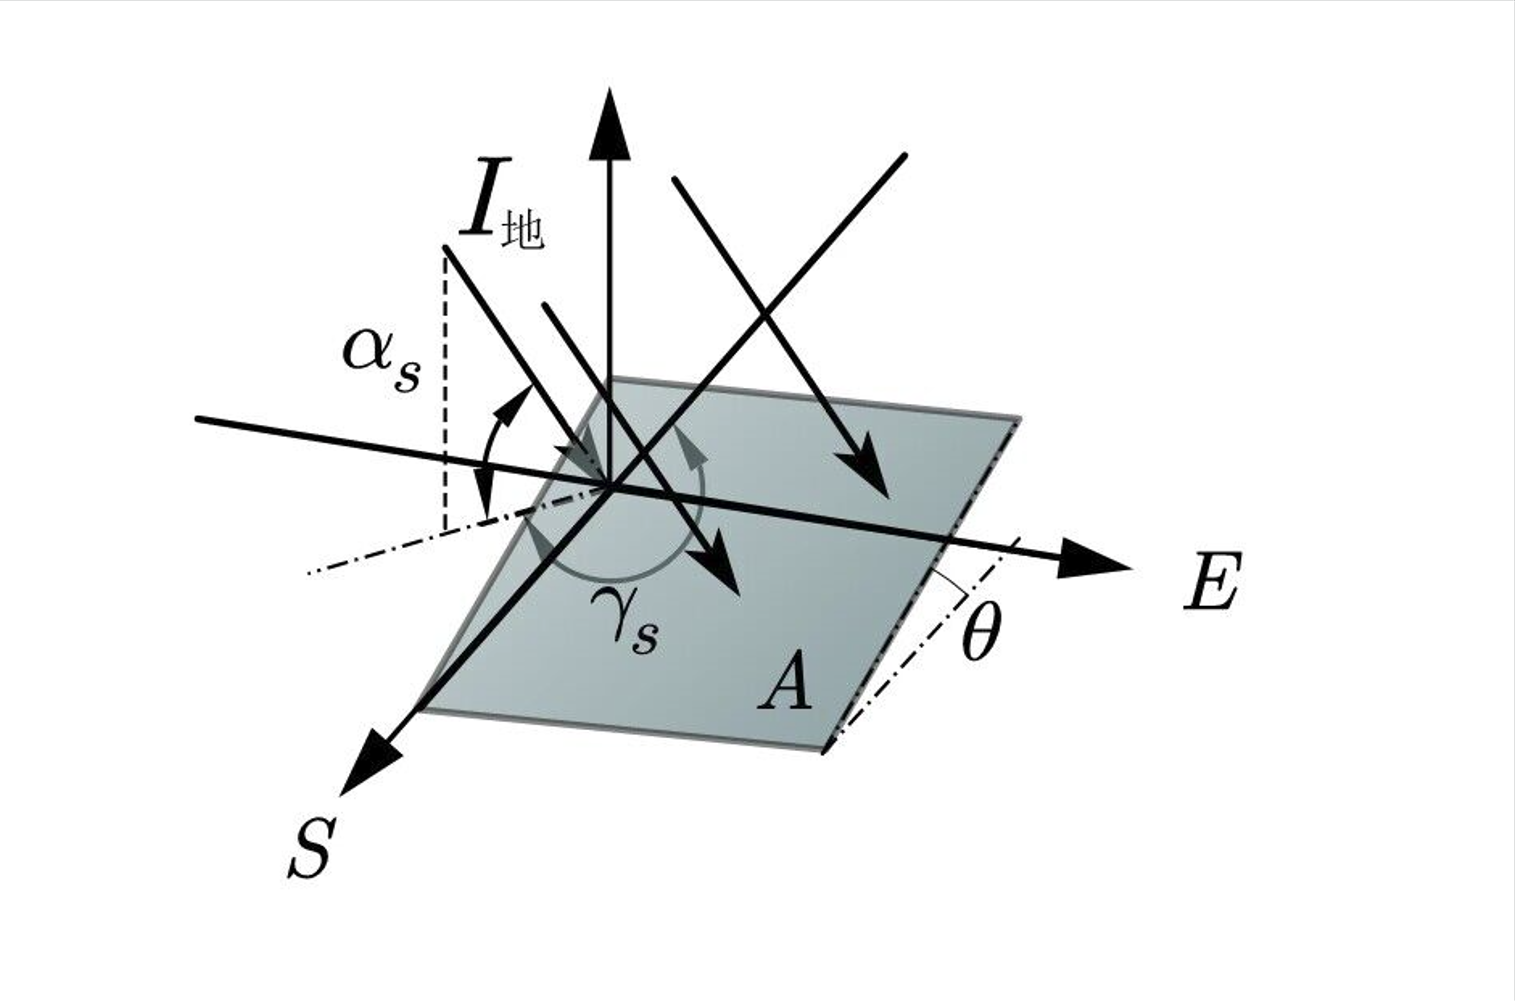
\includegraphics[width=.75\textwidth]{xyz.png}
	\caption{坐标系}
	\label{fig:002}
\end{figure}

由图我们可以得到单位太阳直射的方向向量,这里将方向调转,便于后面余弦效率的计算:

\begin{equation}
	\overrightarrow{I} = (-\cos \alpha_{s}\cos y_{s}, \cos \alpha_{s}\sin y_{s},\sin \alpha_{s})
	\label{eq:004}
\end{equation}

因为光伏板存在水平仰角$\theta$和方位角$\mu$根据题目,水平仰角是光伏电池板平面与水平面的夹角,方位角为光伏板的法线在水平面上的投影与正南方向的夹角。在经过了旋转之后,单位面法向量为:
\begin{equation}
	\overrightarrow{n} = (\sin \theta \cos \mu,\sin \theta \sin \mu,\cos \theta)
	\label{eq:004}
\end{equation}

\begin{figure}
	\centering
	\begin{minipage}[c]{0.48\textwidth}
		\centering
		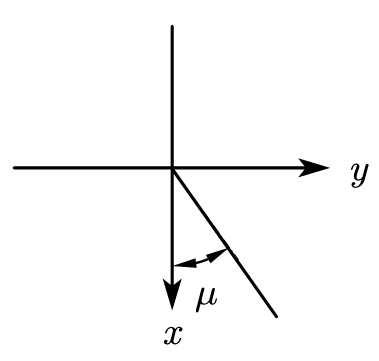
\includegraphics[height=0.2\textheight]{list1.png}
		\subcaption{001}
	\end{minipage}
	\begin{minipage}[c]{0.48\textwidth}
		\centering
		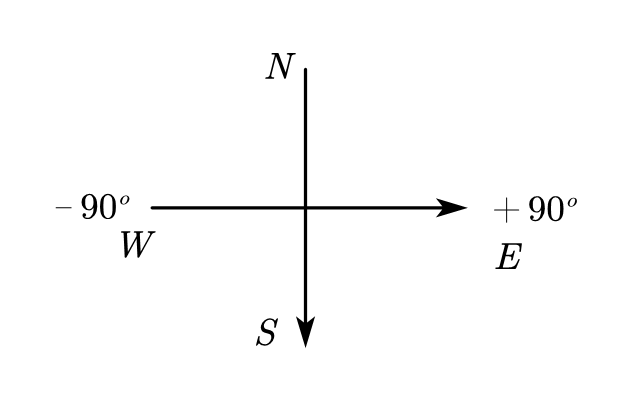
\includegraphics[height=0.2\textheight]{list2.png}
		\subcaption{002}
	\end{minipage}
	\caption{基本角度定义}
\end{figure}

太阳直射辐射照在大气层过后,会被大气层削弱辐射量,其辐射衰减变化量$\Delta I$与大气层厚度$h$成正比,和辐射强度也成正比,大气透射率为穿过大气层的辐射量占总辐射量的百分比,可以得到式子:
\begin{equation}
	\begin{cases}
		\Delta I = kI_{i}h \\
		\eta_{at} = \frac{I_{i} - \Delta I}{I_{i}} = 1-kh 
	\end{cases}
	\label{eq:012}
\end{equation}

再由附录计算5月份的数据来得到该地区的衰减系数:

\begin{equation}
	(1-kh)I_{\mbox{外5月}} = \frac{\sum_{i = 1}^{n} I_{\mbox{地5月15}} i}{n}
	\label{eq:013}
\end{equation}

然后计算仰角为20°,40°,60°的太阳直射光伏板的强度,由大气层外层太阳直射强度经过大气层衰减,再在光伏板上有一定的余弦损失,得到公式:
\begin{equation}
	I_{\mbox{板}}^{(K)(ST)} = I_{\mbox{外i}} * {\eta_{at}} * \eta_{cvs}^{(K)}
	\label{eq:013}
\end{equation}


我们得到结论:在晴天条件下,该城区一块面积为$1m^2$的光伏板朝向正南方且水平倾角分别为20度、40度、60度时受到的最大太阳直射强度和太阳直射辐射总能量如下:

根据当前时刻下的大气层外太阳直射强度得到光伏板方位角为$\theta$时,光伏板水平仰角分别为20度,40度,60度时对应的太阳直射强度:
\begin{table}[!ht]
	\centering
	\begin{tabular}{|l|l|l|l|}
		\hline
		max & 20度 & 40度 & 60度  \\ \hline
		1 & 671.8927023 & 772.5306269 & 780.1873183  \\ \hline
		2 & 718.6440439 & 781.0706871 & 749.3737477  \\ \hline
		3 & 753.7516944 & 767.5017898 & 688.6798423  \\ \hline
		4 & 759.2221365 & 718.0877229 & 590.3413322  \\ \hline
		5 & 740.917085 & 659.4533957 & 498.4500723  \\ \hline
		6 & 720.3452901 & 621.0644194 & 446.8969022  \\ \hline
		7 & 721.4248489 & 631.449314 & 465.3238998  \\ \hline
		8 & 737.2481978 & 681.2664127 & 543.1138437  \\ \hline
		9 & 737.6125263 & 732.266081 & 638.5975392  \\ \hline
		10 & 710.5087563 & 757.6484613 & 713.4480473  \\ \hline
		11 & 668.3074352 & 758.8129613 & 757.9640086  \\ \hline
		12 & 648.0517082 & 758.2021533 & 777.1074906  \\ \hline
	\end{tabular}
\end{table}


\newpage

再对每一个时间段直射能量求和得到不同光伏板倾角的的太阳直射辐射总能量E:
\begin{equation}
	E_{\mbox{光}}^{(k)} = \frac{1}{6} \sum_{6*6}^{18*6} I_{\mbox{板}}^{(k)(ST)} \times (15 \times 60) \times A
	\label{eq:014}
\end{equation}

其中,每个月份不同角度对应的能量如下表所示:

\begin{table}[!ht]
	\centering
	\begin{tabular}{|l|l|l|l|}
		\hline
		月份 & 20度 & 40度 & 60度  \\ \hline
		1 & 15307.28083 & 18408.20635 & 19288.83051  \\ \hline
		2 & 16554.68499 & 18469.94473 & 18157.45655  \\ \hline
		3 & 17571.98231 & 17977.51741 & 16214.69858  \\ \hline
		4 & 17921.20678 & 16625.40956 & 13324.34258  \\ \hline
		5 & 17655.72093 & 15110.39781 & 10742.53771  \\ \hline
		6 & 17245.83912 & 14149.52881 & 9346.576508  \\ \hline
		7 & 17233.85965 & 14425.61417 & 9877.426725  \\ \hline
		8 & 17467.18265 & 15711.78338 & 12061.31116  \\ \hline
		9 & 17271.54399 & 17085.61125 & 14838.90164  \\ \hline
		10 & 16426.06726 & 17867.72101 & 17154.26391  \\ \hline
		11 & 15264.28818 & 18051.25144 & 18660.96736  \\ \hline
		12 & 14711.42173 & 18107.49253 & 19319.5325  \\ \hline
	\end{tabular}
\end{table}

最后,我们将以上表格绘制成折线图,更加直观地看到不同月份之间的太阳辐射强度差异。


\newpage
\begin{figure}
	\centering
	\begin{minipage}[c]{0.45\textwidth}
		\centering
		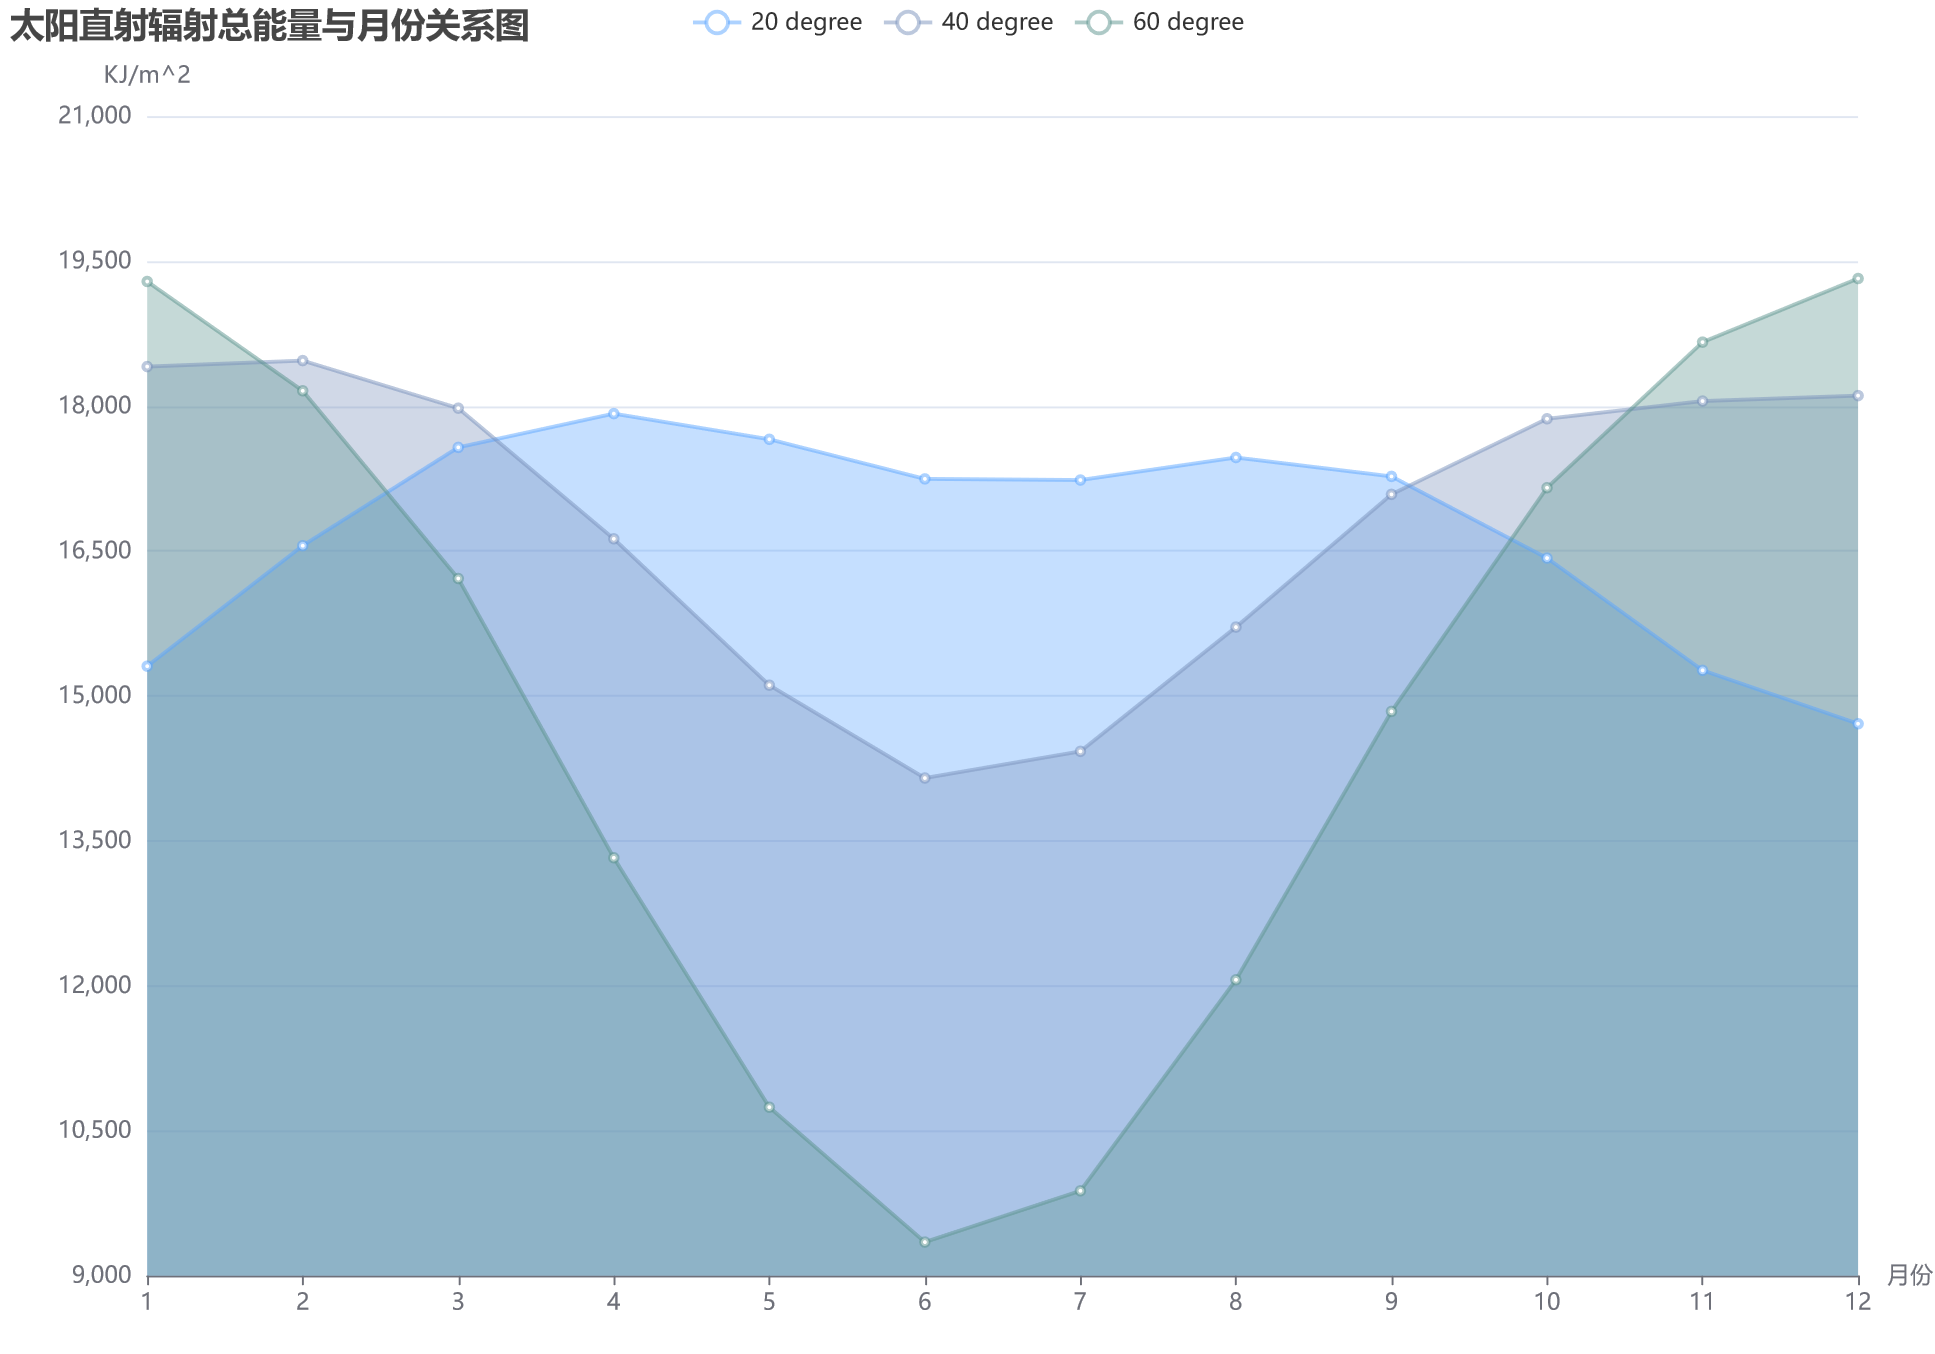
\includegraphics[height=0.19\textheight]{太阳直射辐射总能量与月份关系图.png}
		\subcaption{太阳直射辐射总能量与月份关系图}
	\end{minipage}
	\begin{minipage}[c]{0.45\textwidth}
		\centering
		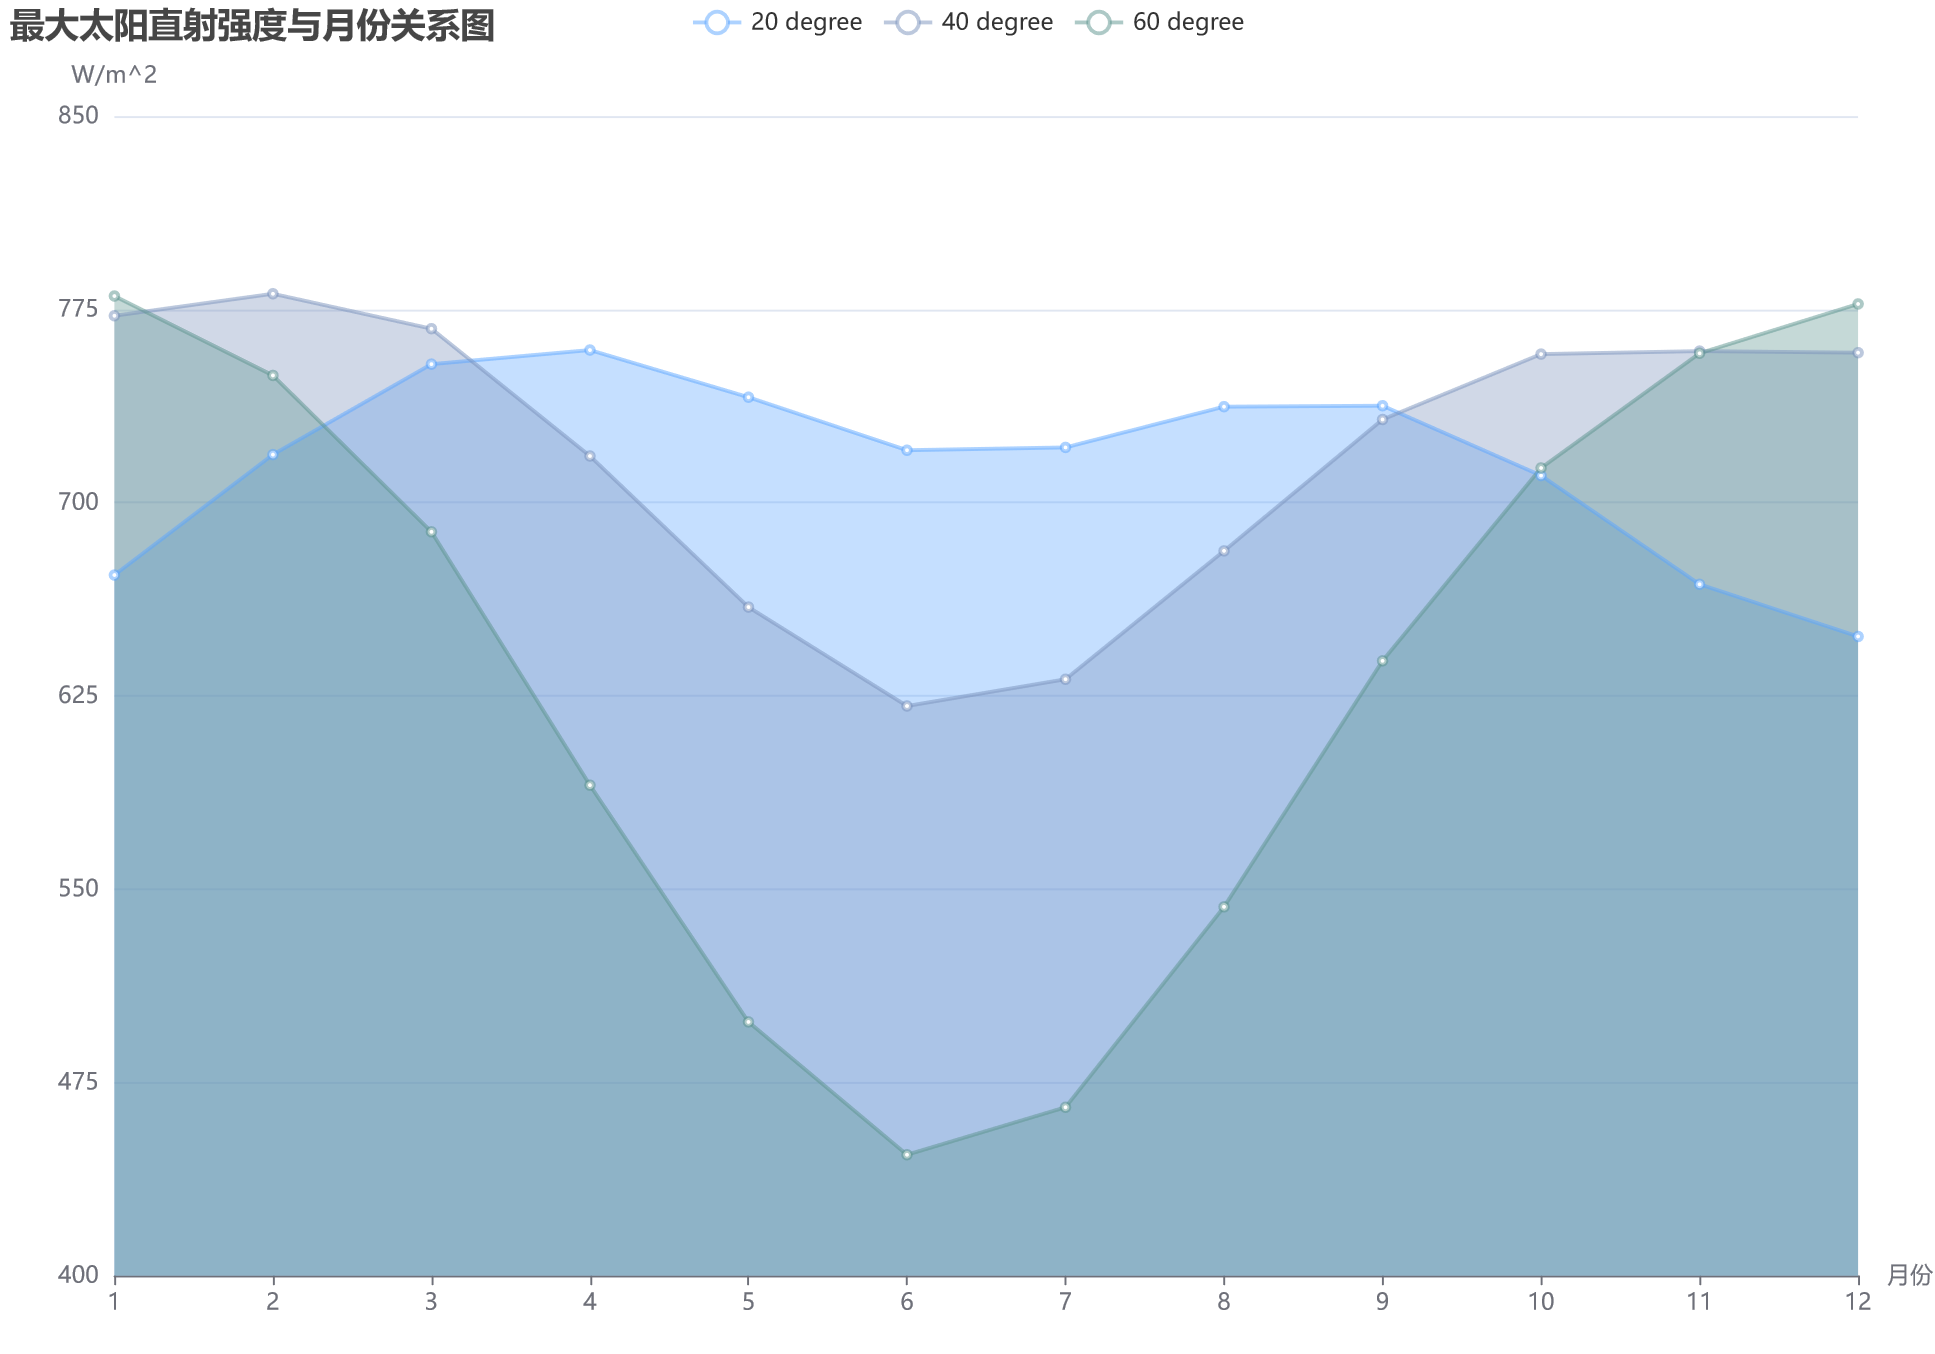
\includegraphics[height=0.19\textheight]{最大太阳直射强度与月份关系图.png}
		\subcaption{最大太阳直射强度与月份关系图}
	\end{minipage}
	\caption{辐射总能量与月份关系图}
\end{figure}

\subsection{问题二}

问题一中我们仅仅讨论每月15日当天光伏板方位角为0时,光伏板水平仰分别为20度,40度,60度下的太阳直射强度和太阳直射辐射总能量,接下来我们要考虑全年平均的情况下,寻找最佳光伏板倾斜角度。

首先,我们得先得到全年晴天时太阳直射地球大气层外表的直射强度,上一问中我们已经得到了该地区的大气层衰减系数,现在我们发现衰减率一直是一个常数,那就是说地面的直射强度和大气层外的直射强度是一个线性关系,那么我们已知5月15日的太阳地面直射强度和每个月的平均大气层外直射强度,则可以根据线性关系把5月15日的太阳直射强度线性映射到一年的每一天中,规定一个月每一天的直射强度都近似相等。

然后再更改$\theta$和$\mu$的值观察光伏板的直射光强和直射辐射总能量的变化,找到最佳点:
\begin{equation}
	\begin{cases}
		I = I(\theta,\mu) \\
		E_{\mbox{光}} = E_{\mbox{光}}(\theta, \mu)
	\end{cases}
	\label{eq:003}
\end{equation}

得到如下三维图,我们寻找鞍点,得到一年中固定太阳能光伏板的最佳的$\theta$和$\mu$:$\theta = 32^{\circ},\mu = 18^{\circ},I_J = 17266 KJ/m2,time = 9.2500$

\begin{figure}
	\centering
	\begin{minipage}[c]{0.48\textwidth}
		\centering
		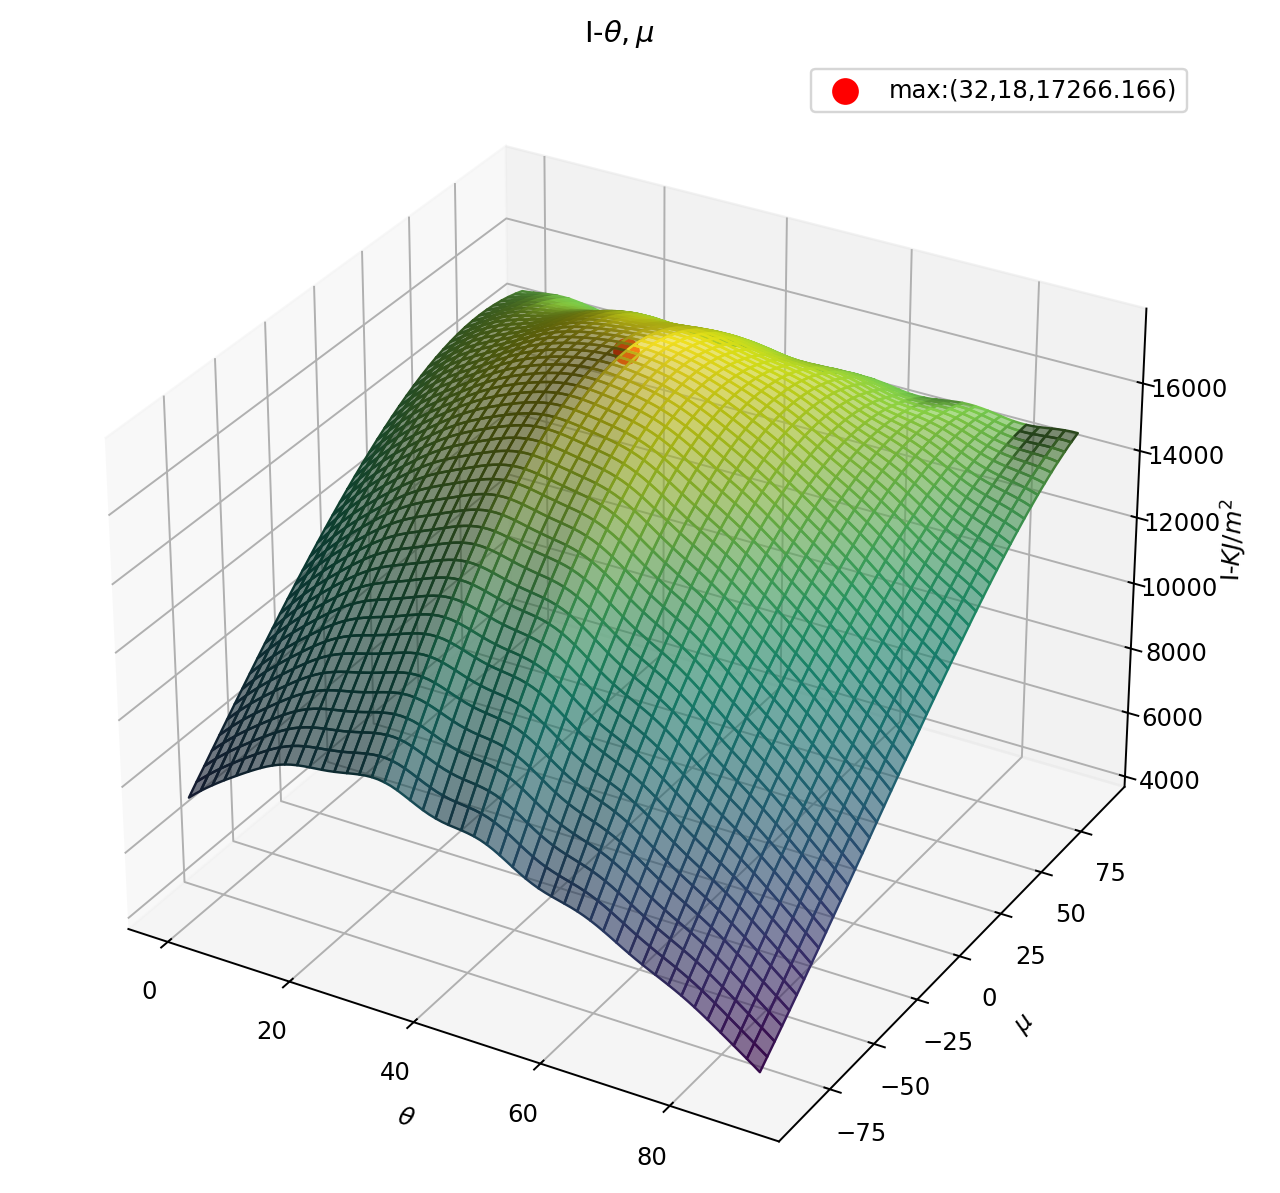
\includegraphics[height=0.22\textheight]{ans3-最大太阳直射辐射平均值.png}
		\subcaption{001}
	\end{minipage}
	\begin{minipage}[c]{0.48\textwidth}
		\centering
		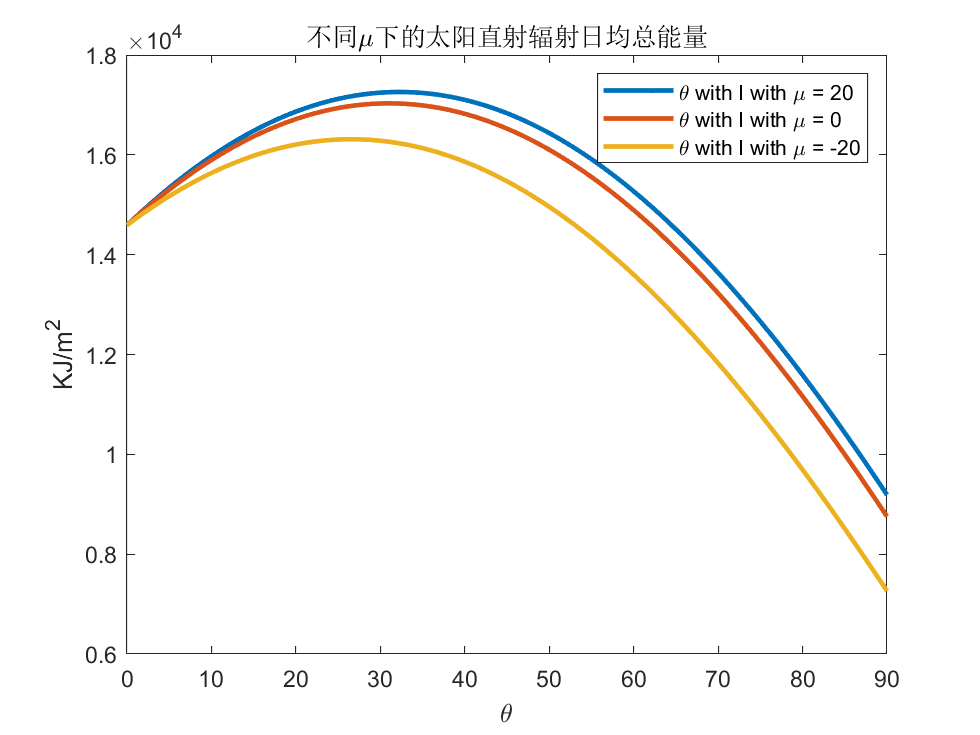
\includegraphics[height=0.2\textheight]{ans2-不同mu下太阳直射辐射日均总能量.png}
		\subcaption{002}
	\end{minipage}
	\caption{问题二}
\end{figure}
\newpage



\subsection{问题三}

当光板受到太阳直射强度过低时,它转换电能的效率也很低;而当光伏板受到太阳直射强度过高时,它转换电能实现储电的效率也会受到限制。我们根据文献得到简化模型的光电转化的效率公式:

\begin{equation}
	\eta = (1-e^{\alpha T})\eta_{STC}\left[ 1-\beta\left( 1-\frac{I}{I_{STC}} \right) \right]
	\label{eq:013}
\end{equation}

其中,ηt为光强转化发热功率的发电效率,ηSTC为标准测试下(光强为1kW/m2,温度为25℃)下的效率。我们进一步得到储电功率:

\begin{equation}
	P_{储} = \eta I
	\label{eq:013}
\end{equation}

其中I为当前时刻的光伏板的太阳直射强度。接着每个时段的储电功率相加得到以一天的储电量,每个时段为15分钟:

\begin{equation}
	C = \sum_{6*6}^{36*6} (P_{\mbox{储}} - P_{\mbox{放}}) \times (15 \times 60)
	\label{eq:013}
\end{equation}


为了考虑路灯蓄电池的储电效率高和储电量大这两个目标,接下来我们利用基于熵权法的TOPSIS算法,分析光伏板受到太阳直射强度上午大于150 W/m2,下午大于100 W/m2的时间,以及一天的储电量来设计出光伏板固定安装的最优朝向。



我们引入熵权法+TOPSIS评价的方法,利用熵权法客观赋权,借鉴了信息熵思想,通过计算指标的信息熵,根据指标的相对变化程度对系统整体的影响来决定指标的权重进行赋权,然后根据所得到的权重,进行TOPSIS评价。
基于熵权的光伏板固定朝向综合评价TOPSIS法可分为以下5步:

第1步:采用向量规范化的方法构造决策矩阵X。采用n个评价单元、m个评价指标的光伏板固定朝向综合评价问题。其中我们有三个评价指标,分别为:有阳光直射光伏板的强度上午大于$150W/m^2$的时间,下午大于$150W/m^2$的时间,以及光伏板一天的储电量,建立决策矩阵X为:

\begin{equation}
	X_{ij}=\left ( X_{ij} \right )_{m\times n}
	\label{eq:013}
\end{equation}

式中: xij 表示第i个评价单元的第j个评价指标值,其中i n = 1, …,n  ; j = 1,… ,3

第2步:对决策矩阵X进行正向化和标准化处理。首先对评价指标进行正向化处理:



\begin{equation}
	X_{ij}^{'}=\frac{X_{ij}^{}-min\left \{ X_{ij} \right \}}{max\left \{ X_{ij} \right \}-min\left \{ X_{ij} \right \}}+0.0001
	\label{eq:013}
\end{equation}

再将正向化后的指标标准化,以去除量纲对决策矩阵的影响



\begin{equation}
(Z_{ij})_{m\times n}=\frac{R_{ij}'}{\sqrt{\sum_{i=1}^{m}R_{ij}^{2}}}
	\label{eq:013}
\end{equation}



第3步:采用熵权模型前,采用标准差对各个指标的离散程度进行初步判断,若满足熵权的使用条件,采用熵权模型确定每个指标的熵权值,计算信息效用值,并归一化得到每个指标的熵权值;若不满足,则采用层次分析法对权重进行修正,采用主客观结合的方式提高了模型的适应性。

首先计算各评价指标的标准差判断各指标的离散程度:





\begin{equation}
	s_{ij} = \sqrt{ s^2 } = \sqrt{ \frac{\sum_{i=1}^{n}(z_{ij}-\bar{z})^2}{n-1}}
	\label{eq:013}
\end{equation}


若满足评价指标的标准差不为零,或者标准差的值比较大,即各评价指标的数据存在一定的差异性和波动性。这意味着指标之间具有一定的差异,可以通过权衡它们的重要性来进行熵权的计算。则可以采用熵权法计算步骤如下:计算概率矩阵P:






\begin{equation}
	\left ( P_{ij} \right )_{m\times n}=\frac{X_{ij}^{'}}{\sum_{i=1}^{m}X_{ij}^{'}}
	\label{eq:013}
\end{equation}



对于第j个指标,其信息熵为:





\begin{equation}
	e_{j}=-k\sum_{i=1}^{m}P_{ij}lnP_{ij}   \quad    k=\frac{1}{lnm}
	\label{eq:013}
\end{equation}



确定信息效用值:







\begin{equation}
g_{j}=1-e_{j}
	\label{eq:013}
\end{equation}



将信息效用值进行归一化,确定每个指标的熵权:





\begin{equation}
	W{j}=\frac{g_{i}}{\sum_{j=1}^{n}}g_{j}
	\label{eq:013}
\end{equation}


若不满足则采用层次分析法对权重进行修正。经过计算,我们的数值满足熵权法的使用条件,因此以下不列出层次分析法的权重修正。


第 4 步:计算各决策方案到正理想解的距离 $Di+$ 和负理想距离 $Di-$






\begin{equation}
	D_{i}^{-}=\sqrt{\sum_{j=1}^{n}(Z_{j}^{-}-Z_{ij})^2} \qquad D_{i}^{+}=\sqrt{\sum_{j=1}^{n}(Z_{j}^{+}-Z_{ij})^2}
	\label{eq:013}
\end{equation}



第 5 步:计算各方案的排序指标值 Si (即评价指数),按 Si由大到小排列方案的优劣次序。计算第 i 个评价对象未归一化的得分:




\begin{equation}
	C_{i}=\frac{D_{i}^{-}}{D_{i}^{+}+D_{i}^{-}}
	\label{eq:013}
\end{equation}

将得分进行归一化:




\begin{equation}
	C_{i} = \frac{D_{i}^{-}}{D_{i}^{+} + D_{i}^{-}}
	\label{eq:013}
\end{equation}


以上构成确定光伏板性能等级的基于熵权的光伏板固定朝向综合评价TOPSIS法。

我们以储电量,上午大于$150W/m^2$的时长,下午大于$100W/m^2$的时长三者作为评价指标,根据前两问,利用matlab模拟得到,三者与$\theta$,$\mu$的关系

最终得到对应的权值
\begin{table}[!ht]
	\centering
	\begin{tabular}{|l|l|l|}
		\hline
		储电量 & 上午大于$150W/m^2$的时长 &  下午大于$100W/m^2$的时长 \\ \hline
		0.3317 & 0.3306 & 0.3323 \\ \hline
	\end{tabular}
\end{table}

根据权值,再结合TOPSIS法,进行评价,通过矩阵运算算出最后的得分结果,最终得到,$\theta = 32,\mu = 18,I_J = 17266 KJ/m2,time = 9.2500$
\begin{figure}
	\centering
	\begin{minipage}[c]{0.3\textwidth}
		\centering
		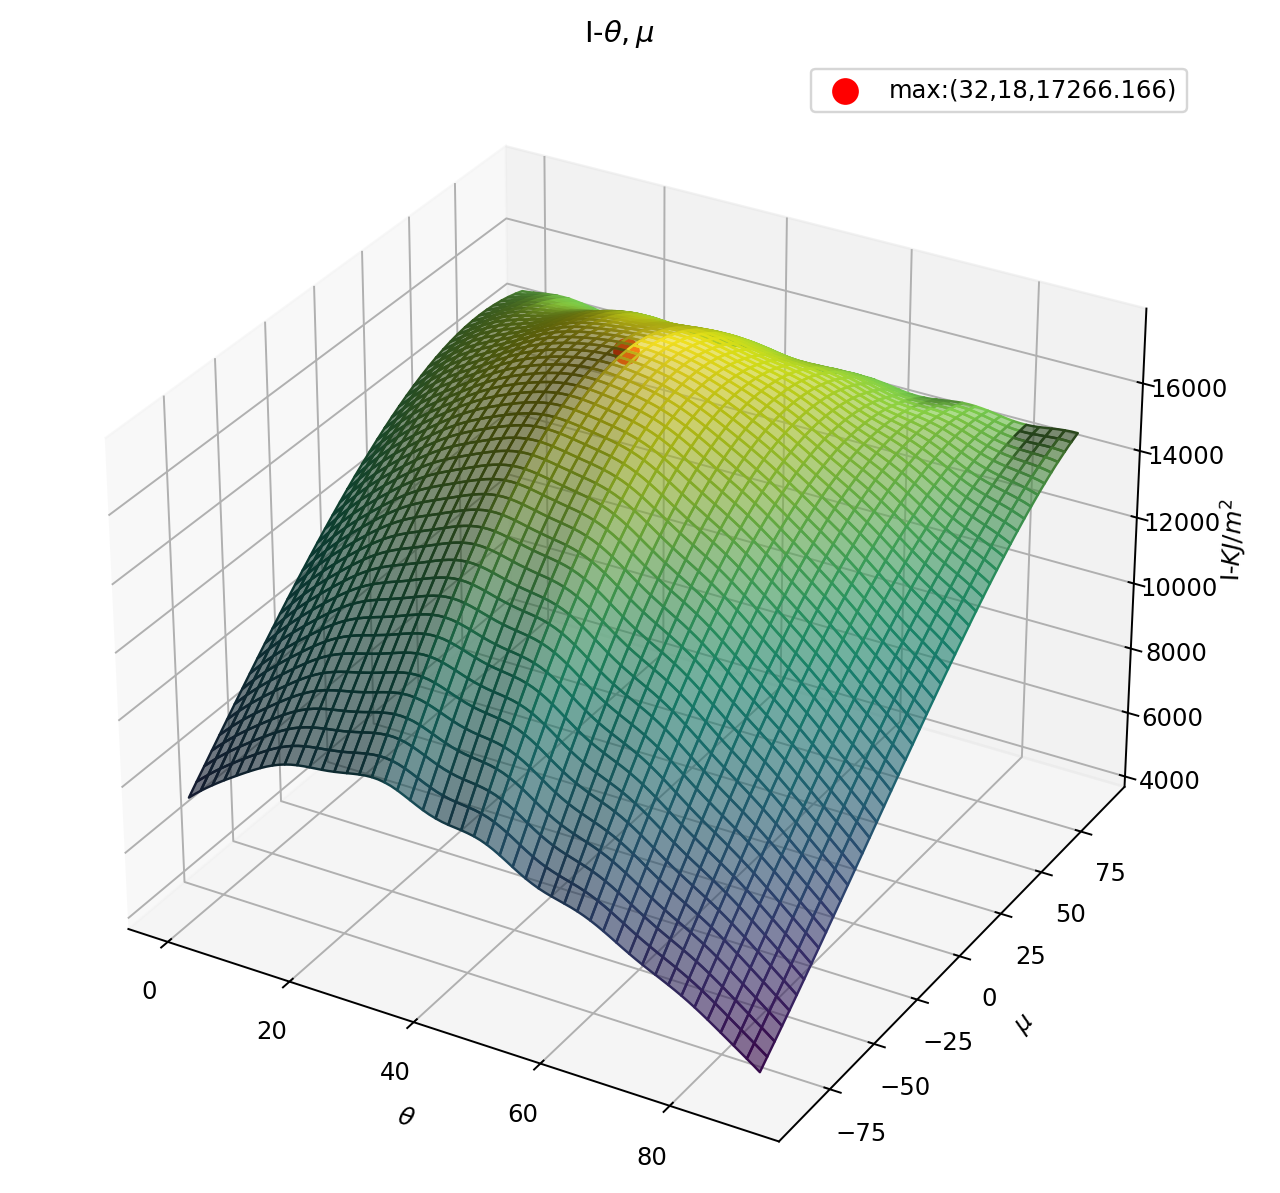
\includegraphics[height=0.2\textheight]{ans3-最大太阳直射辐射平均值.png}
		\subcaption{储电量}
	\end{minipage}
	\begin{minipage}[c]{0.3\textwidth}
		\centering
		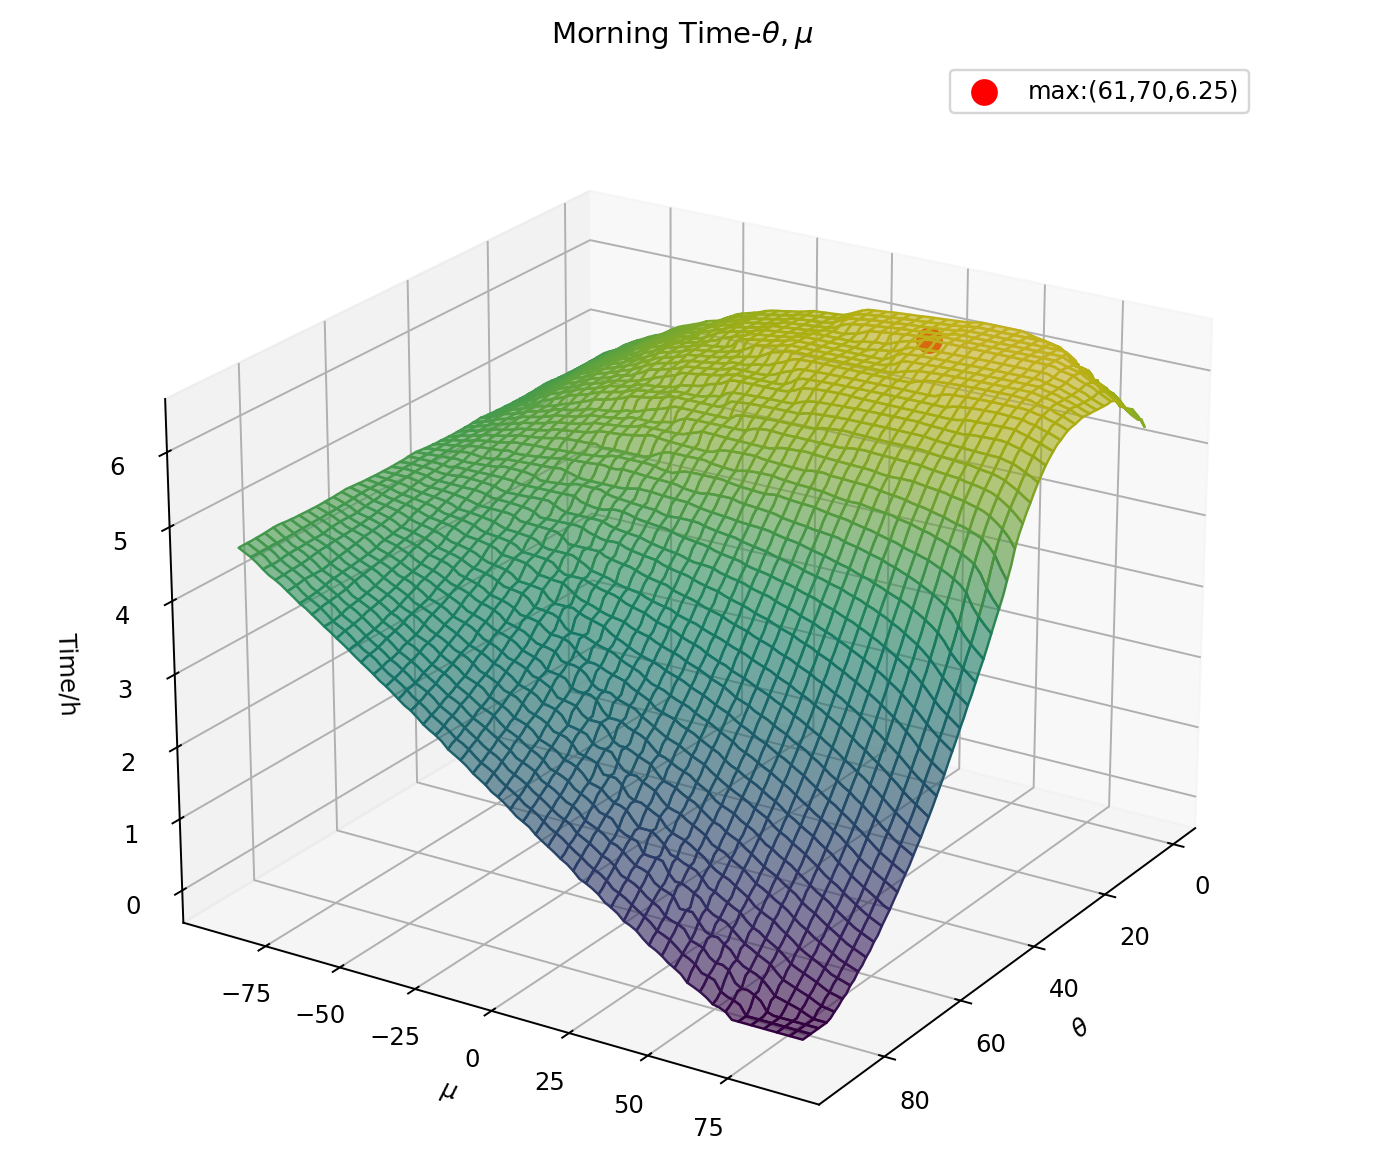
\includegraphics[height=0.2\textheight]{ans3-morning.png}
		\subcaption{上午时长}
	\end{minipage}
	\begin{minipage}[c]{0.3\textwidth}
		\centering
		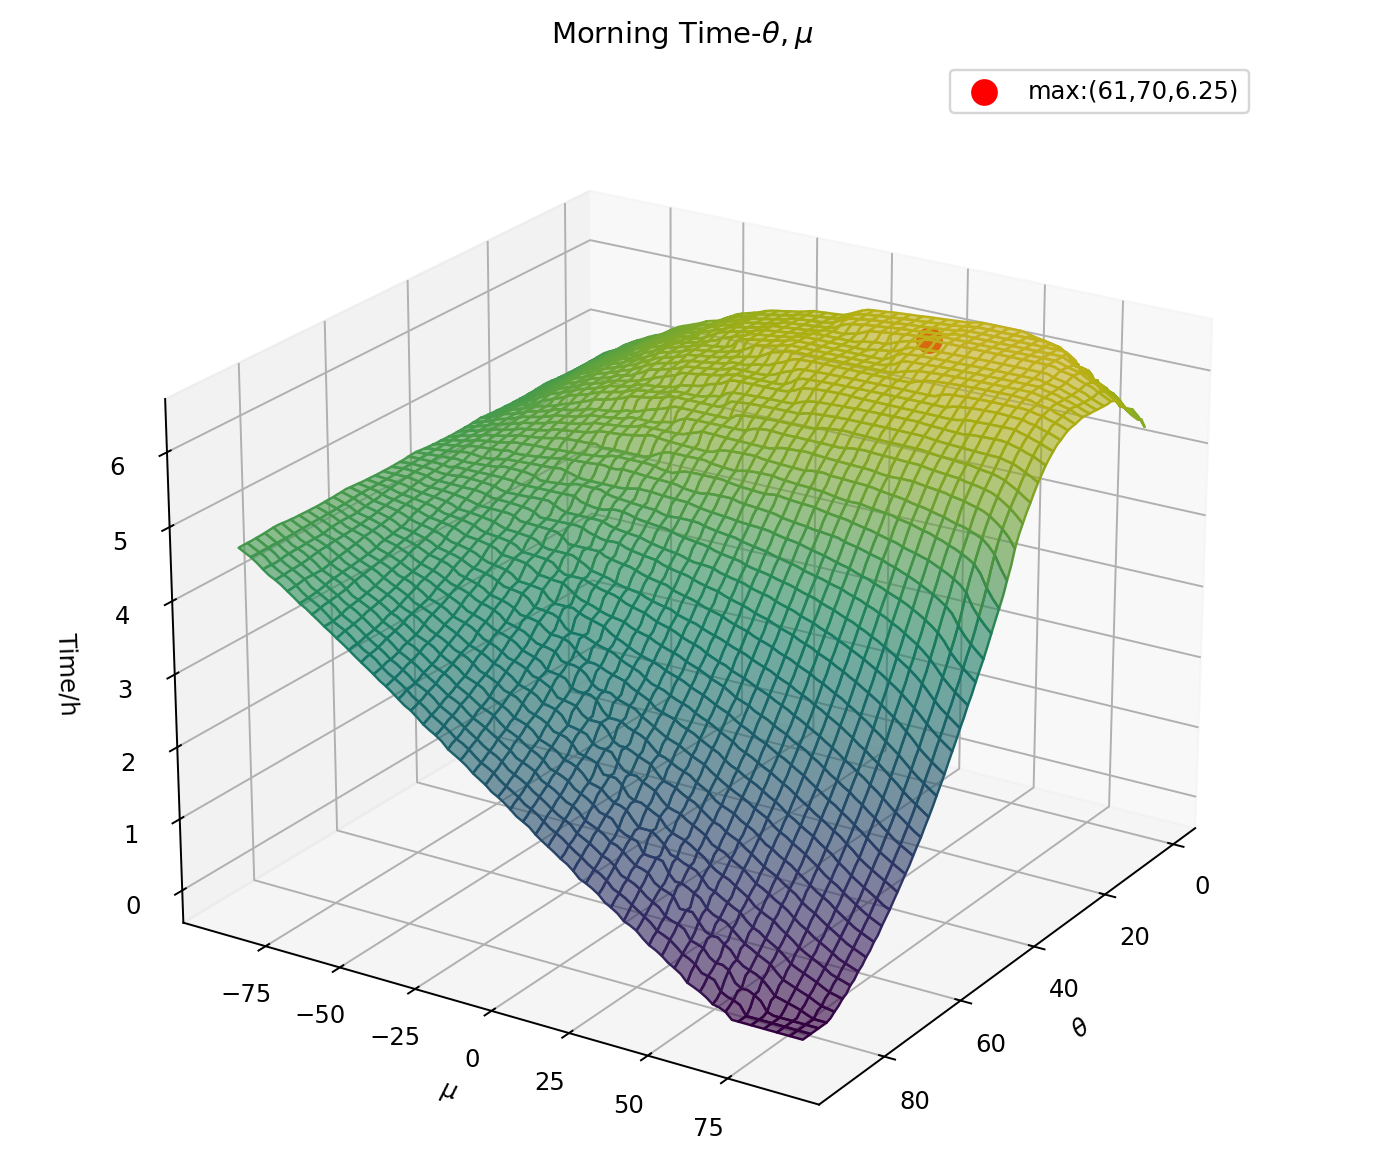
\includegraphics[height=0.2\textheight]{ans3-morning.png}
		\subcaption{下午时长}
	\end{minipage}
\end{figure}


\begin{figure}[!h]
	\centering
	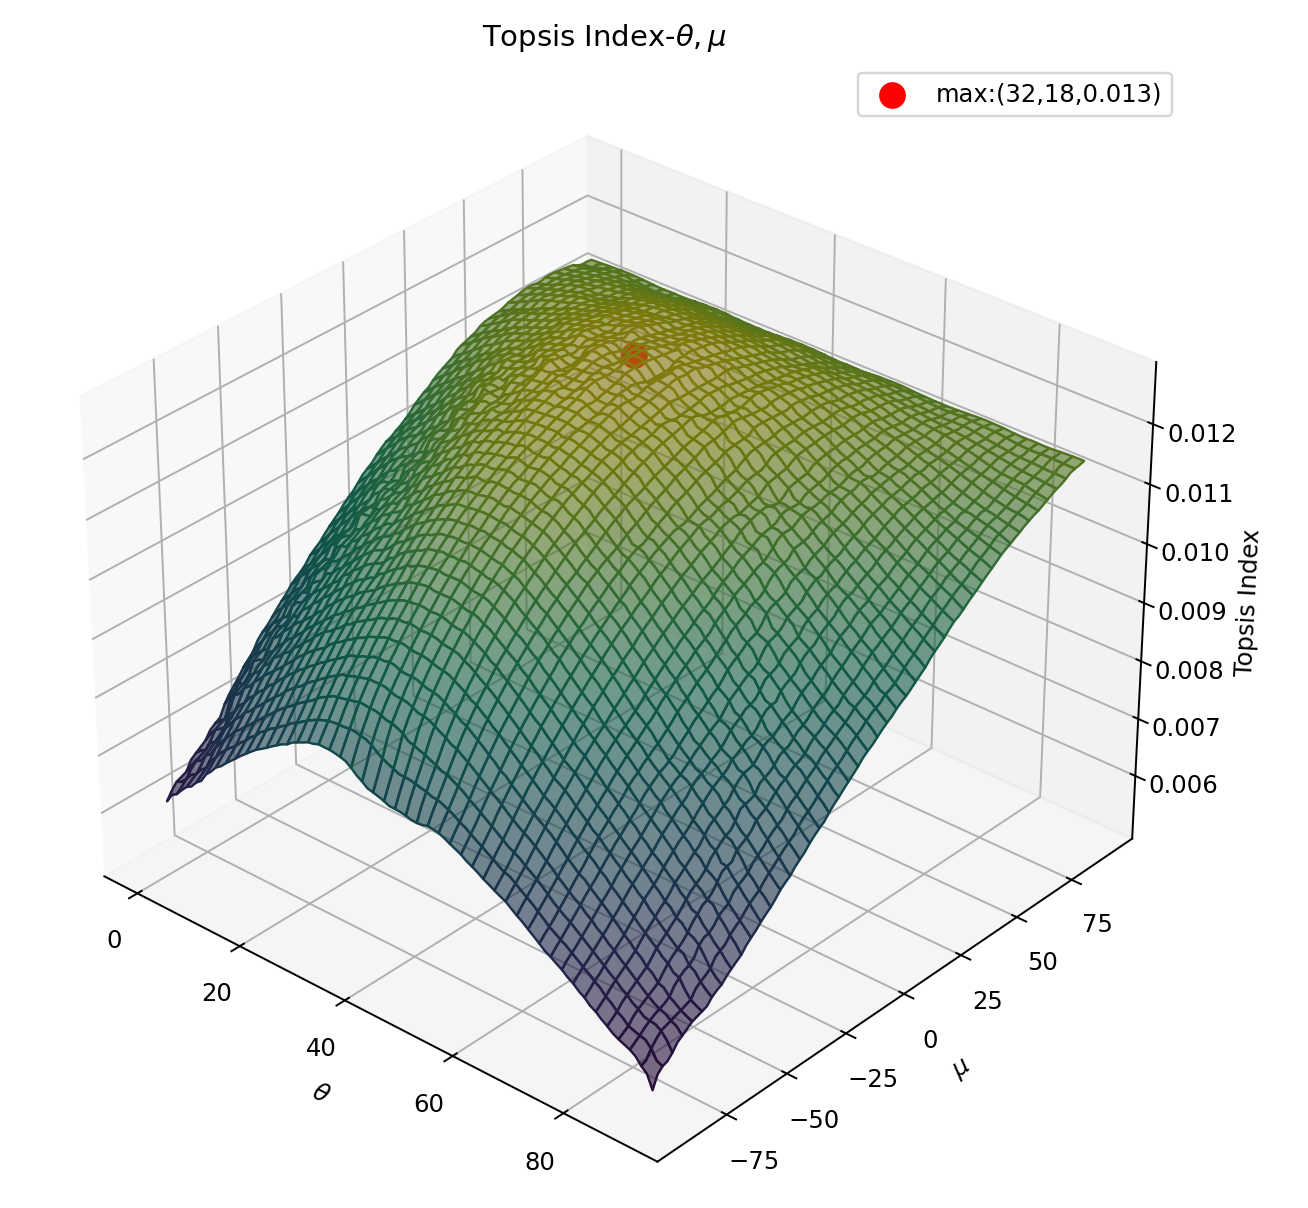
\includegraphics[width=.5\textwidth]{ans3-topsis.png}
	\caption{TOPSIS评价指数}
	\label{fig:002}
\end{figure}



\begin{figure}[!h]
	\centering
	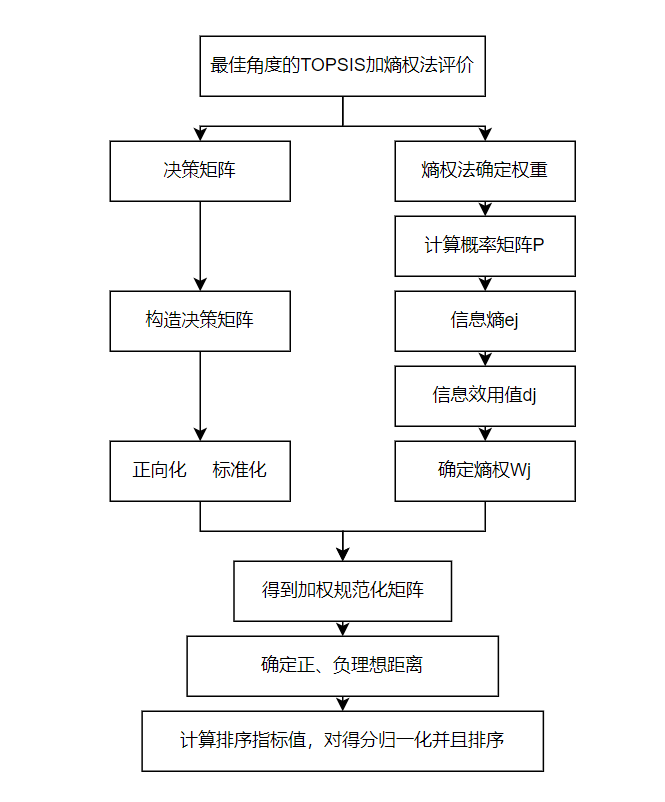
\includegraphics[width=.5\textwidth]{流程.png}
	\caption{流程图}
	\label{fig:002}
\end{figure}


\newpage

\section{模型评价与推广运用}

\subsection{模型评价}

\subsubsection{模型优点}
\begin{enumerate}
	\item 本模型在Klein-Theilacker模型的基础上,结合实际,引入了光伏转化效率与电池储存效率,对模型进行改进,综合考虑了光伏板的角度因素与转化、储存效率因素。
	\item 由于所给数据较少,故对原始数据进行了插值,提高了模型的精度。
	\item 引入熵权法加TOPSIS评价模型,利用熵权法客观的权重,来评价最佳方案,用于选择综合考虑光强与效率时的最佳角度。
\end{enumerate}

\subsubsection{模型缺点与改进}
\begin{enumerate}
	\item 模型忽略了温度的影响。由于温度会影响材料的物理特性,比如电阻、光伏转化效率、电池活性等,从而影响到太阳能的接收和储存效率。模型应该结合不同月份的典型温度,取添加温度修正项,从而考虑温度的影响。
	\item 只考虑了晴天条件,忽略了气象因素。这导致模型的适用性较差。所以,应该要结合当地的气象数据,通过历年的气象数据统计,从而增添相关的气象因素,修正模型。
	\item 当前模型可能未考虑城市环境因素对太阳辐射的影响,如建筑物的遮挡、地形的起伏等。在未来可以通过数字地图和三维城市模型来模拟城市环境,以更准确地估计光伏板受到的太阳辐射,从而增加模型的实用性。
\end{enumerate}

\subsection{推广运用}

本文主要讨论了光伏板最佳摆放角度的问题,设计了光伏板角度与光伏板收集最大辐射能模型,并且利用基于熵权法与TOPSIS方法的评估模型,找到最佳角度。在能源领域上,可以参考该模型,结合当地的气象数据来获得光伏板的最佳摆放角度,从而得到最大发电效率,提高全年的发电量,为能源的利用提供支持。并且,由于该模型同时得到了最差的角度,即受到阳光照射影响最小的角度,所以在某些需要避开阳光紫外线影响建筑外墙设计过程中,可以参考此模型,达到提高材料寿命,节省成本的目的。此外,本文设计的模型还可以应用于可变角度的光伏板中,由于在某些特殊情况下,例如卫星、太空探测器的光伏板角度可调的情况下,可以利用该模型让角度始终保持在最佳,从而使得最终获得的总太阳辐射能最大。综上所述,本文设计的模型具有比较广泛的实际应用价值,能够在利用、避免幅射光的领域中起到一定贡献的作用。

\newpage

\section{参考文献与引用}

%参考文献
\begin{thebibliography}{9}%宽度9
    \bibitem{1}姚天亮, 吴兴全. 基于光照强度曲线微积分的光伏发电特性分析[J]. Advances in Energy and Power Engineering, 2018, 6: 131.
    \bibitem{2}黄伟, 张田, 韩湘荣, 等. 影响光伏发电的日照强度时间函数和气象因素[J]. 电网技术, 2014, 38(10): 2789-2793.
    \bibitem{3}尤海侠. 光伏发电效率影响因素分析[J]. 能源技术与管理,2022,47(6):147-149. DOI:10.3969/j.issn.1672-9943.2022.06.046.
    \bibitem{4}尚华,王惠荣. 太阳能光伏发电效率的影响因素[J]. 宁夏电力,2010(5):48-50,57. DOI:10.3969/j.issn.1672-3643.2010.05.015.
    \bibitem{5}16家主流企业光伏电池效率一览. https://guangfu.bjx.com.cn/news/20231204/1347414.shtml
    \bibitem{6}陈维,沈辉,邓幼俊. 太阳能光伏应用中的储能系统研究[J]. 蓄电池,2006,43(1):21-27. DOI:10.3969/j.issn.1006-0847.2006.01.005.
    \bibitem{7}SYNODINOU, B. M., \& KATSOULIS, B. D. (1996). A COMPARISON OF THREE MODELS FOR ESTIMATION OF GLOBAL SOLAR IRRADIATION ON TILTED AND ORIENTED SURFACES IN ATHENS. International Journal of Solar Energy, 18(2), 83–102. https://doi.org/10.1080/01425919608914308
\end{thebibliography}

\newpage







%附录
\begin{appendices}

\section{支撑材料文件列表}

\begin{table}[!htbp]
	\label{tab:001} \centering
	\setlength{\tabcolsep}{25mm}
	\begin{tabular*}{\hsize}{@{}@{\extracolsep{\fill}}l@{}}
		\toprule[1.5pt]
		\qquad 文件名列表 \\
		\midrule[1pt]
		\qquad \textbf{Latex源文件} \\
		\qquad \textbf{img} \\
		\qquad \textbf{参考论文} \\
		\qquad \qquad  不同方位倾斜面上太阳辐射量及最佳倾角的计算\_杨金焕.pdf\\
		\qquad \qquad  固定式光伏方阵最佳倾角的分析\_杨金焕.pdf\\
		\qquad \qquad  固定式太阳能光伏板最佳倾角设计方法研究.pdf\\
		\qquad \qquad  光伏发电效率影响因素分析.pdf\\
		\qquad \qquad  基于光照强度曲线微积分的光伏发电特性分析.pdf\\
		\qquad \qquad  太阳能光伏发电效率的影响因素\_尚华.pdf\\
		\qquad \qquad  太阳能光伏应用中的储能系统研究.pdf\\
		\qquad \qquad  影响光伏发电的日照强度时间函数和气象因素.pdf\\
		\qquad \qquad  A COMPARISON OF THREE MODELS.pdf\\
		\qquad \textbf{源程序代码}\\
		\qquad \qquad \textbf{问题一} \\
		\qquad \qquad \qquad q1.m \\
		\qquad \qquad \qquad interp.m \\
		\qquad \qquad \qquad origin.xlsx \\
		\qquad \qquad \qquad interp.xlsx \\
		\qquad \qquad \qquad answer1.xlsx \\
		\qquad \qquad \textbf{问题二} \\
		\qquad \qquad \qquad q2.m \\
		\qquad \qquad \qquad pro2.xlsx \\
		\qquad \qquad \qquad answer2.py \\
		\qquad \qquad \qquad interp.xlsx \\
		\qquad \qquad \textbf{问题三} \\
		\qquad \qquad \qquad q3.m \\
		\qquad \qquad \qquad interp.xlsx \\
		\qquad \qquad \qquad C\_m.xlsx \\
		\qquad \qquad \qquad c2.xlsx \\
		\qquad \qquad \qquad t\_afternoon.xlsx \\
		\qquad \qquad \qquad t\_morning.xlsx \\
		\qquad \qquad \qquad ans3.txt \\
		\qquad \qquad \qquad answer3.py \\
		\bottomrule[1.5pt]
	\end{tabular*}
\end{table}





\newpage



\section{补充表格、图片和公式推导}

\textbf{插值后结果}

\begin{table}[!ht]
	\centering
	\begin{tabular}{|l|l|l|l|l|l|}
		\hline
		time & I  & time & I  & time & I  \\ \hline
		0.25 & 21.132  & 0.447923 & 732.0782533  & 0.645846 & 605.2472271  \\ \hline
		0.260417 & 43.01970038  & 0.45834 & 736.6073811  & 0.656263 & 575.8122758  \\ \hline
		0.270834 & 64.90889811  & 0.468757 & 741.8905502  & 0.66668 & 546.3628342  \\ \hline
		0.281251 & 110.1933472  & 0.479174 & 747.1710627  & 0.677097 & 505.6070301  \\ \hline
		0.291668 & 155.479052  & 0.489591 & 748.680611  & 0.687514 & 464.8471677  \\ \hline
		0.302085 & 210.574815  & 0.500008 & 750.1907388  & 0.697931 & 421.071767  \\ \hline
		0.312502 & 265.6702883  & 0.510425 & 752.4548112  & 0.708348 & 377.2836154  \\ \hline
		0.322919 & 319.257003  & 0.520842 & 754.7201396  & 0.718765 & 324.4519248  \\ \hline
		0.333336 & 372.8462295  & 0.531259 & 758.4937603  & 0.729182 & 271.5902386  \\ \hline
		0.343753 & 436.2447582  & 0.541676 & 762.2558854  & 0.739599 & 198.3803959  \\ \hline
		0.35417 & 499.6370075  & 0.552093 & 753.1990956  & 0.750016 & 125.2238786  \\ \hline
		0.364587 & 543.4119083  & 0.56251 & 744.1459283  & 0.760433 & 86.7321469  \\ \hline
		0.375004 & 587.180723  & 0.572927 & 738.8627593  & 0.77085 & 48.2718112  \\ \hline
		0.385421 & 615.1061166  & 0.583344 & 733.5672249  & 0.781267 & 29.40320742  \\ \hline
		0.395838 & 643.0291434  & 0.593761 & 716.2081694  & ~ & ~ \\ \hline
		0.406255 & 665.6713679  & 0.604178 & 698.843366  & ~ & ~ \\ \hline
		0.416672 & 688.3120467  & 0.614595 & 676.2011415  & ~ & ~ \\ \hline
		0.427089 & 707.9351746  & 0.625012 & 653.5571781  & ~ & ~ \\ \hline
		0.437506 & 727.5496084  & 0.635429 & 629.4054147  & ~ & ~ \\ \hline
	\end{tabular}
\end{table}










 \section{源程序代码}
\textbf{模型一}

q1.m\quad \& \quad interp.m
\begin{lstlisting}[language=matlab]
	
%q1.m
%%
clear;clc;
filename = "interp.xlsx";
[num,txt,~] = xlsread(filename);
%%
clc;
monthI = [1405,1394,1378,1353,1334,1316,1308,1315,1330,1350,1372,1392];
startDay = datetime('2024-3-21');

nowDay = datetime('2024-12-15'); % 当前日期
nowHour = 12; % 当前时间

w = pi/12*abs(12-nowHour);

%latitude = 35/360*2*pi;
latitude = 30.583/360*2*pi; % latitude in rad

D = days(nowDay-startDay);

delta = asin(sin(2*pi*D/365)*sin(2*pi/360*23.45)); % delta in rad 与当前日期有关

% 太阳高度角 alpha_s in rad 与当前日期与当前时间有关
alpha_s = asin(cos(delta)*cos(latitude)*cos(w)+sin(delta)*sin(latitude)); 

disp(alpha_s*360/2/pi)

kh = 0.6864; % ***待定***
eta_at = 1 - kh; 

theta_k = [0,20,40,60]*2*pi/360;

eta_cos = sin(theta_k+alpha_s);

mu = 0/360*2*pi;

y_s = asin((sin(delta)-sin(alpha_s)*sin(latitude))/(cos(alpha_s)*cos(latitude)));

%%
% Answer 1
clc;
I = zeros(12,4); % I(a,b,c) a是月份,b是角度
sin_y_s = 0;
temp = [0,0,0,0];
maxI = zeros(12,3);
for i = 1:12
temp = [0,0,0,0];
nowDay = nowDay + calmonths(1); % 计算当前日期
%disp(nowDay)
D = days(nowDay-startDay); % 更新日期差
delta = asin(sin(2*pi*D/365)*sin(2*pi/360*23.45));
disp("Month:" + i)
for j = 1:48 % 从早上6点到晚上18点
nowHour = 6 + 0.25*j;
w = pi/12*(nowHour-12);
alpha_s = asin(cos(delta)*cos(latitude)*cos(w)+sin(delta)*sin(latitude));
cos_y_s = (sin(delta)-(sin(alpha_s) * sin(latitude))) / (cos(alpha_s) * cos(latitude));
if nowHour >= 12
sin_y_s = - sqrt(1-cos_y_s*cos_y_s);
else 
sin_y_s = sqrt(1-cos_y_s*cos_y_s);
end
eta_cos = -cos(alpha_s)*cos_y_s*sin(theta_k)*cos(mu)+cos(alpha_s)*sin_y_s*sin(theta_k)
*sin(mu)+sin(alpha_s)*cos(theta_k);
%y_s = asin((sin(delta)-sin(alpha_s)*sin(latitude))/(cos(alpha_s)*cos(latitude)));
%disp(y_s*360/2/pi);
%disp("Time:" +nowHour+ " "+ sin(alpha_s) + " " + cos(alpha_s) + " " + sin(y_s) + " " + cos(y_s))
disp("Time:" +nowHour+ " " + sin_y_s);
%disp(" ("+(-cos(alpha_s)*cos(y_s))+","+cos(alpha_s)*sin(y_s)+","+sin(alpha_s)+")")
if num(j,2)*(monthI(month(nowDay))/1334)*15*60*eta_cos>=0
temp = temp + num(j,2)*(monthI(month(nowDay))/1334)*15*60*eta_cos;
end
maxI(i,1) = max(maxI(i,1),num(j,2)*(monthI(month(nowDay))/1334)*eta_cos(2));
maxI(i,2) = max(maxI(i,2),num(j,2)*(monthI(month(nowDay))/1334)*eta_cos(3));
maxI(i,3) = max(maxI(i,3),num(j,2)*(monthI(month(nowDay))/1334)*eta_cos(4));
end
I(i,:) = temp;
end

I = I/1000;
plot(1:12,I(:,2),"LineWidth",2,"DisplayName","20 degree")
hold on;
plot(1:12,I(:,3),"LineWidth",2,"DisplayName","40 degree")
hold on;
plot(1:12,I(:,4),"LineWidth",2,"DisplayName","60 degree")
hold on;
xlabel("month")
ylabel("KJ/m^{2}")
legend

%%%%%%%%%%%%%%%%%%%%%%%%%%%%

%interp.m

%%
clear;clc;
filename = "1.xlsx";
[num,txt,~] = xlsread(filename);
newX = 0.25:0.010417:0.79;
newY = interp1(num(:,1),num(:,2),newX,'spline');
scatter(newX.*24,newY,'red',"filled","o",'DisplayName',"The light intensity with interpolation",SizeData=15);
xlabel("Time",FontSize=16)
ylabel("I",FontSize=16)
hold on;
scatter(num(:,1).*24,num(:,2),'blue',"filled","o","DisplayName","Origin Data",SizeData=20);
legend;

%%
% export
colName = ["time","I"];
k = [newX;newY]';
T = array2table(k, 'VariableNames', colName);
writetable(T, "interp.xlsx", 'Sheet', 1, 'Range', 'A1');

k = ["["+num(:,1).*24+",",num(:,2)+"],"];
T = array2table(k, 'VariableNames', colName);
writetable(T, "origin.xlsx", 'Sheet', 1, 'Range', 'A1');
%%

 \end{lstlisting}


\textbf{模型二}

answer2.py
\begin{lstlisting}[language=python]	
	import openpyxl
	import numpy as np
	import matplotlib.pyplot as plt
	from mpl_toolkits.mplot3d import Axes3D
	
	# 打开Excel文件
	workbook = openpyxl.load_workbook("pro2.xlsx")
	
	# 选择第一个工作表
	sheet = workbook.active
	
	# 获取工作表的行数和列数
	rows = sheet.max_row
	columns = sheet.max_column
	
	# 创建二维列表用于存储数据
	a = [[None] * columns for _ in range(rows)]
	
	# 遍历Excel表格中的所有单元格,并将值存储在a列表中
	for index_row, row in enumerate(sheet.iter_rows(min_row=1, max_row=rows, min_col=1, max_col=columns), start=0):
	for index_column, cell in enumerate(row, start=0):
	if str(cell.value).find("i"):
	try:
	a[index_row][index_column] = complex(str(cell.value).replace("i", "j").replace(' ','')).real
	except ValueError:
	print(cell.value)
	input()
	else :
	a[index_row][index_column] = float(str(cell.value))
	a = np.array(a)
	
	max_index = np.unravel_index(np.argmax(a), a.shape)
	print("最大值的下标为:", max_index)
	
	# 获取数组的维度
	rows, cols = a.shape
	x = np.arange(0, cols)
	y = np.arange(0, rows)
	x, y = np.meshgrid(x, y)
	
	fig = plt.figure()
	ax = fig.add_subplot(111, projection='3d')
	
	colors = plt.cm.viridis((a - np.min(a)) / (np.max(a) - np.min(a)))
	
	ax.plot_surface(x, y*2-90, a/1000, alpha=0.6,facecolors=colors)
	
	ax.scatter(xs=38, ys=-22, zs=a[32][36]/1000+5,s=100, marker='o',color='red', label='max:(32,-18,'+str(int(a[32][36]/1000))+')')
	ax.set_xlabel(r'$\theta$')
	ax.set_ylabel(r'$\mu$')
	ax.set_zlabel(r'I-$KW/m^2$')
	plt.legend()
	plt.show()
	
\end{lstlisting}

q2.m
\begin{lstlisting}[language=matlab]
	%%
	clear;clc;
	filename = "interp.xlsx";
	[num,txt,~] = xlsread(filename);
	%%
	clc;
	monthI = [1405,1394,1378,1353,1334,1316,1308,1315,1330,1350,1372,1392];
	startDay = datetime('2024-3-21');
	
	nowDay = datetime('2024-12-15'); % 当前日期
	nowHour = 12; % 当前时间
	
	w = pi/12*abs(12-nowHour);
	
	%latitude = 35/360*2*pi;
	latitude = 30.583/360*2*pi; % latitude in rad
	
	D = days(nowDay-startDay);
	
	delta = asin(sin(2*pi*D/365)*sin(2*pi/360*23.45)); % delta in rad 与当前日期有关
	
	% 太阳高度角 alpha_s in rad 与当前日期与当前时间有关
	alpha_s = asin(cos(delta)*cos(latitude)*cos(w)+sin(delta)*sin(latitude)); 
	
	disp(alpha_s*360/2/pi)
	
	kh = 0.6864; % ***待定***
	eta_at = 1 - kh; 
	
	theta_k = [0,20,40,60]*2*pi/360;
	
	eta_cos = sin(theta_k+alpha_s);
	
	mu = 0/360*2*pi;
	
	y_s = asin((sin(delta)-sin(alpha_s)*sin(latitude))/(cos(alpha_s)*cos(latitude)));
	
	%%
	% Answer 2
	temp = 0;
	sin_y_s = 0;
	nowDay = datetime('2023-12-31');
	I_theta = zeros(91,1);
	theta_k0 = 0;
	for mu_360 = -20:20:20
	temp = 0;
	sin_y_s = 0;
	nowDay = datetime('2023-12-31');
	I_theta = zeros(91,1);
	theta_k0 = 0;
	mu = mu_360*2*pi/360;
	for theta_k0_360 = 0:1:90
	theta_k0 = theta_k0_360*2*pi/360; 
	temp = 0;
	for i = 1:365
	nowDay = nowDay + days(1); % 当前日期
	D = days(nowDay-startDay); % 更新日期差
	delta = asin(sin(2*pi*D/365)*sin(2*pi/360*23.45));
	for j = 1:48 % 从早上6点到晚上18点
	nowHour = 6 + 0.25*j;
	w = pi/12*(nowHour-12);
	alpha_s = asin(cos(delta)*cos(latitude)*cos(w)+sin(delta)*sin(latitude));
	%if j == 24
	%disp(i + " " + alpha_s*360/2/pi);
	%end
	cos_y_s = (sin(delta)-(sin(alpha_s) * sin(latitude))) / (cos(alpha_s) * cos(latitude));
	if nowHour >= 12
	sin_y_s = - sqrt(1-cos_y_s*cos_y_s);
	else 
	sin_y_s = sqrt(1-cos_y_s*cos_y_s);
	end
	eta_cos = -cos(alpha_s)*cos_y_s*sin(theta_k0)*cos(mu)+cos(alpha_s)*sin_y_s*sin(theta_k0)*sin(mu)+sin(alpha_s)*cos(theta_k0);
	temp = temp + num(j,2)*(monthI(month(nowDay))/1334)*15*60*eta_cos/365;
	end
	end
	%disp(theta_k0_360+" " +temp);
	I_theta(fix(theta_k0_360)+1,:) = temp;
	end
	plot(0:1:90,I_theta/1000,"LineWidth",2,"DisplayName","\theta with I with \mu = "+num2str(-mu_360));
	hold on;
	end
	xlabel("\theta")
	ylabel("KJ/m^{2}")
	title("不同\mu下的太阳直射辐射日均总能量")
	legend
	
	%%
	% Answer 2 3D
	temp = 0;
	sin_y_s = 0;
	nowDay = datetime('2023-12-31');
	I_theta = zeros(91,91,1);
	theta_k0 = 0;
	for mu_360 = -90:2:90
	mu_rad = mu_360*2*pi/360;
	for theta_k0_360 = 0:1:90
	theta_k0 = theta_k0_360*2*pi/360; 
	temp = 0;
	for i = 1:365
	nowDay = nowDay + days(1); % 当前日期
	D = days(nowDay-startDay); % 更新日期差
	delta = asin(sin(2*pi*D/365)*sin(2*pi/360*23.45));
	for j = 1:48 % 从早上6点到晚上18点
	nowHour = 6 + 0.25*j;
	w = pi/12*(nowHour-12);
	alpha_s = asin(cos(delta)*cos(latitude)*cos(w)+sin(delta)*sin(latitude));
	%if j == 24
	%disp(i + " " + alpha_s*360/2/pi);
	%end
	cos_y_s = (sin(delta)-(sin(alpha_s) * sin(latitude))) / (cos(alpha_s) * cos(latitude));
	if nowHour >= 12
	sin_y_s = - sqrt(1-cos_y_s*cos_y_s);
	else 
	sin_y_s = sqrt(1-cos_y_s*cos_y_s);
	end
	eta_cos = -cos(alpha_s)*cos_y_s*sin(theta_k0)*cos(mu_rad)+
	cos(alpha_s)*sin_y_s*sin(theta_k0)*sin(mu_rad)+sin(alpha_s)*cos(theta_k0);
	temp = temp + num(j,2)*(monthI(month(nowDay))/1334)*15*60*eta_cos/365;
	end
	end
	%disp(theta_k0_360+" " +temp);
	I_theta(fix(theta_k0_360)+1,fix((mu_360+90)/2)+1,:) = temp;
	end
	end
	
\end{lstlisting}



\textbf{模型三}

q3.m
\begin{lstlisting}[language=matlab]
	%%
	clear;clc;
	filename = "interp.xlsx";
	[num,txt,~] = xlsread(filename);
	%%
	clc;
	monthI = [1405,1394,1378,1353,1334,1316,1308,1315,1330,1350,1372,1392];
	startDay = datetime('2024-3-21');
	
	nowDay = datetime('2024-12-15'); % 当前日期
	nowHour = 12; % 当前时间
	
	w = pi/12*abs(12-nowHour);
	
	%latitude = 35/360*2*pi;
	latitude = 30.583/360*2*pi; % latitude in rad
	
	D = days(nowDay-startDay);
	
	delta = asin(sin(2*pi*D/365)*sin(2*pi/360*23.45)); % delta in rad 与当前日期有关
	
	% 太阳高度角 alpha_s in rad 与当前日期与当前时间有关
	alpha_s = asin(cos(delta)*cos(latitude)*cos(w)+sin(delta)*sin(latitude)); 
	
	disp(alpha_s*360/2/pi)
	
	kh = 0.6864; % ***待定***
	eta_at = 1 - kh; 
	
	theta_k = [0,20,40,60]*2*pi/360;
	
	eta_cos = sin(theta_k+alpha_s);
	
	mu = 0/360*2*pi;
	
	y_s = asin((sin(delta)-sin(alpha_s)*sin(latitude))/(cos(alpha_s)*cos(latitude)));
	
	%%
	% Answer 3
	I_board = 1000;
	I_STC = 1000;
	beta = 0.5;
	eta_STC = 0.15;
	eta_t = eta_STC*(1-beta*(1-I_board/I_STC));
	
	temp = 0;
	temp_morning = 0;
	temp_afternoon = 0;
	sin_y_s = 0;
	nowDay = datetime('2023-12-31');
	I_theta = zeros(91,91,3);
	theta_k0 = 32*2*pi/360;
	for mu_360 = -90:2:90
	mu_rad = mu_360*2*pi/360;
	for theta_k0_360 = 0:1:90
	theta_k0 = theta_k0_360*2*pi/360; 
	temp = 0;
	temp_morning = 0;
	temp_afternoon = 0;
	for i = 1:365
	nowDay = nowDay + days(1); % 当前日期
	D = days(nowDay-startDay); % 更新日期差
	delta = asin(sin(2*pi*D/365)*sin(2*pi/360*23.45));
	for j = 1:48 % 从早上6点到晚上18点
	nowHour = 6 + 0.25*j;
	w = pi/12*(nowHour-12);
	alpha_s = asin(cos(delta)*cos(latitude)*cos(w)+sin(delta)*sin(latitude));
	cos_y_s = (sin(delta)-(sin(alpha_s) * sin(latitude))) / (cos(alpha_s) * cos(latitude));
	if nowHour >= 12
	sin_y_s = - sqrt(1-cos_y_s*cos_y_s);
	else 
	sin_y_s = sqrt(1-cos_y_s*cos_y_s);
	end
	eta_cos = -cos(alpha_s)*cos_y_s*sin(theta_k0)*cos(mu_rad)+
	cos(alpha_s)*sin_y_s*sin(theta_k0)*sin(mu_rad)+sin(alpha_s)*cos(theta_k0);
	I_board = num(j,2)*(monthI(month(nowDay))/1334)*eta_cos;
	if nowHour >= 12
	if I_board >= 150
	temp_morning = temp_morning + 1;
	end
	else
	if I_board >= 100
	temp_afternoon = temp_afternoon + 1;
	end
	end
	eta_t = eta_STC*(1-beta*(1-I_board/I_STC));
	if I_board >= 0
	temp = temp + I_board*15*60/365;
	end
	end
	end
	%disp(theta_k0_360+" " +temp);
	I_theta(fix(theta_k0_360)+1,fix((mu_360+90)/2)+1,1) = temp;
	I_theta(fix(theta_k0_360)+1,fix((mu_360+90)/2)+1,2) = temp_morning/4/365;
	I_theta(fix(theta_k0_360)+1,fix((mu_360+90)/2)+1,3) = temp_afternoon/4/365;
	end
	end
	%%
	
	C_m = real(I_theta(:,:,1));
	t_morning = I_theta(:,:,2);
	t_afternoon = I_theta(:,:,3);
	
	%%
	clc;
	topsis_m = [C_m(:),t_morning(:),t_afternoon(:)]; 
	
	[n,m] = size(topsis_m);
	
	for i=1:n
	for j = 1:m
	if topsis_m(i,j) == 0
	topsis_m(i,j) = 0.001;
	end
	end
	end
	
	topsis_m = topsis_m ./ repmat(sum(topsis_m.*topsis_m).^0.5,n,1);
	
	p = topsis_m ./ sum(topsis_m, 1); % 每列的相对概率分布
	entropy_vals = -sum(p .* log(p), 1); % 计算每列的信息熵
	
	% 计算各指标的权重
	weights = (1 - entropy_vals) / sum(1 - entropy_vals); % 根据信息熵计算权重
	
	c1 = weights*topsis_m';
	c2 = reshape(c1, size(C_m));
\end{lstlisting}

\end{appendices}

\end{document} 